% ==========================================================
% 30-minute seminar --- derived deck
% Generated from the frame library; see DECK_GUIDE.md.
% Frames come from frames/. A frame needing different prose for this talk
% gets its own frames/<id>_talk.tex, listed here instead of the original.
% The macro sections below are THE SPINE, shared with slides_report.tex
% and the paper. A short deck may GLUE adjacent sections; it may never
% reorder, drop, or invent one.
% ==========================================================

\documentclass[aspectratio=169,10pt]{beamer}
% ============================================================
% Shared Beamer preamble — Electoral Judicialization
% ------------------------------------------------------------
% Inputted by BOTH decks, after their own \documentclass:
%   slides_report.tex   — the full research report (canonical)
%   slides_advisor.tex  — the short advisor highlight deck
%
% Holds the house theme, colors, custom commands, and the \input of
% the auto-generated number macros. Deck-specific \title/\author/\date
% stay in each deck file.
%
% The colors here mirror code/utils/figure_style.R's PAL so figures and
% slides match. Change a color HERE, never in one deck only.
% ============================================================

% ---- Theme ----
\usetheme{default}
\useinnertheme{rectangles}
\setbeamertemplate{navigation symbols}{}
\setbeamertemplate{footline}[frame number]

% ---- Packages ----
\usepackage{booktabs}
\usepackage{dcolumn}  % decimal-aligned numeric columns (first-stage table)
\usepackage{amsmath,amssymb}
\usepackage{graphicx}
\usepackage{xcolor}
\usepackage{tikz}
\usetikzlibrary{arrows.meta,shapes.geometric,positioning,fit,backgrounds,calc}
\usepackage{array}
\usepackage{longtable}
\usepackage{multirow}
\usepackage{tabularx}
\usepackage[authoryear,round]{natbib}
\usepackage{hyperref}
\usepackage[utf8]{inputenc}
\usepackage{colortbl}

% ---- Colors ----
\definecolor{myblue}{RGB}{0,90,156}
\definecolor{mydark}{RGB}{55,55,55}
\definecolor{mylight}{RGB}{220,230,242}
\definecolor{myred}{RGB}{180,30,30}
\definecolor{mygreen}{RGB}{0,120,60}
\definecolor{mygray}{RGB}{130,130,130}
\definecolor{sigshade}{RGB}{226,243,230}  % pale green: cells significant at 5%
\definecolor{rowlaw}{RGB}{252,242,242}   % lawsuits: light red
\definecolor{rowcnd}{RGB}{242,246,255}   % candidates: light blue
\definecolor{rowvot}{RGB}{242,252,245}   % votes: light green
\definecolor{rowctl}{RGB}{250,250,250}   % controls: light gray
\definecolor{rownws}{RGB}{255,248,235}   % news: light amber
% category band colors (stronger tints for header rows)
\definecolor{bandlaw}{RGB}{232,205,205}
\definecolor{bandcnd}{RGB}{205,218,240}
\definecolor{bandvot}{RGB}{208,235,216}
\definecolor{bandctl}{RGB}{228,228,228}
\definecolor{bandnws}{RGB}{245,228,196}

% Make \dagger from auto-generated etable fragments safe in text mode
\let\latexdagger\dagger
\renewcommand{\dagger}{\ensuremath{\latexdagger}}

\setbeamercolor{frametitle}{bg=myblue,fg=white}
\setbeamercolor{title}{fg=white,bg=myblue}
\setbeamercolor{subtitle}{fg=mylight,bg=myblue}
\setbeamercolor{structure}{fg=myblue}
\setbeamercolor{alerted text}{fg=myred}
\setbeamercolor{block title}{bg=myblue!20,fg=myblue}
\setbeamercolor{block body}{bg=myblue!5}
\setbeamercolor{block title alerted}{bg=myred!20,fg=myred}
\setbeamercolor{block body alerted}{bg=myred!5}
\setbeamerfont{frametitle}{size=\normalsize,series=\bfseries}

% ---- Column types ----
\newcolumntype{L}[1]{>{\raggedright\arraybackslash}p{#1}}
\newcolumntype{C}[1]{>{\centering\arraybackslash}p{#1}}
\newcolumntype{R}[1]{>{\raggedleft\arraybackslash}p{#1}}

% ---- Custom commands ----
\newcommand{\bZ}{\mathit{Z}_{m}^{\textsc{b}}}
\newcommand{\pos}[1]{\textcolor{mygreen}{\textbf{#1}}}
\newcommand{\negt}[1]{\textcolor{myred}{\textbf{#1}}}
\newcommand{\ns}[1]{\textcolor{mydark}{#1}}
\newcommand{\tick}{{\color{mygreen}$\checkmark$}}
\newcommand{\cross}{{\color{myred}$\times$}}

% ---- Takeaway strip: one pale-blue full-width band carrying a frame's single
%      spoken takeaway (usually the per-SD magnitude). Keeps results frames to
%      the grammar: assertion title -> one exhibit -> one takeaway strip. ----
\newcommand{\takeaway}[1]{\par\smallskip{\setlength{\fboxsep}{5pt}%
  \noindent\colorbox{mylight}{\parbox{\dimexpr\linewidth-2\fboxsep\relax}{%
  \footnotesize #1}}}\par}

% ---- Auto-generated numbers — nothing hardcoded ----
% Single source of truth: regenerated by 06_abstract_macros.py after every
% estimation run. Defines first-stage, outcome, descriptive, instrument-
% distribution, universe, exposure-robust, and disaggregated-turnout macros
% used by both decks.
% abstract_macros.tex — auto-generated by 06_abstract_macros.py
% DO NOT EDIT MANUALLY.

\providecommand{\AdvLawsuitsTwenty}{0.05}
\renewcommand{\AdvLawsuitsTwenty}{0.05}
\providecommand{\AdvLawsuitsFortyFour}{0.04}
\renewcommand{\AdvLawsuitsFortyFour}{0.04}
\providecommand{\TotalLawsuitsTwenty}{1.22}
\renewcommand{\TotalLawsuitsTwenty}{1.22}
\providecommand{\NMunisExposedTwenty}{4,419}
\renewcommand{\NMunisExposedTwenty}{4,419}
\providecommand{\ShareMunisExposedTwenty}{79.3}
\renewcommand{\ShareMunisExposedTwenty}{79.3}
\providecommand{\AdvPerCandidateTwenty}{0.1}
\renewcommand{\AdvPerCandidateTwenty}{0.1}
\providecommand{\AdvPerCandidateFortyFour}{0.1}
\renewcommand{\AdvPerCandidateFortyFour}{0.1}
\providecommand{\VotersPerAdvTwenty}{3,149}
\renewcommand{\VotersPerAdvTwenty}{3,149}
\providecommand{\VotersPerAdvFortyFour}{4,071}
\renewcommand{\VotersPerAdvFortyFour}{4,071}
\providecommand{\RegisteredVotersTwenty}{149.42}
\renewcommand{\RegisteredVotersTwenty}{149.42}
\providecommand{\RegisteredVotersFortyFour}{156.47}
\renewcommand{\RegisteredVotersFortyFour}{156.47}
\providecommand{\TurnoutRateTwenty}{76.8}
\renewcommand{\TurnoutRateTwenty}{76.8}
\providecommand{\TurnoutRateFortyFour}{78.3}
\renewcommand{\TurnoutRateFortyFour}{78.3}
\providecommand{\BlankRateTwenty}{3.4}
\renewcommand{\BlankRateTwenty}{3.4}
\providecommand{\BlankRateFortyFour}{2.8}
\renewcommand{\BlankRateFortyFour}{2.8}
\providecommand{\BlankVotesTwenty}{3.94}
\renewcommand{\BlankVotesTwenty}{3.94}
\providecommand{\ExecCandsTwenty}{19,379}
\renewcommand{\ExecCandsTwenty}{19,379}
\providecommand{\ExecCandsFortyFour}{15,574}
\renewcommand{\ExecCandsFortyFour}{15,574}
\providecommand{\LegCandsTwenty}{518,485}
\renewcommand{\LegCandsTwenty}{518,485}
\providecommand{\LegCandsFortyFour}{432,002}
\renewcommand{\LegCandsFortyFour}{432,002}
\providecommand{\FemaleShareExecTwenty}{13.4}
\renewcommand{\FemaleShareExecTwenty}{13.4}
\providecommand{\FemaleShareExecFortyFour}{15.3}
\renewcommand{\FemaleShareExecFortyFour}{15.3}
\providecommand{\NMunis}{5,560}
\renewcommand{\NMunis}{5,560}
\providecommand{\NZones}{26}
\renewcommand{\NZones}{26}
\providecommand{\FSCoef}{0.418}
\renewcommand{\FSCoef}{0.418}
\providecommand{\FSSE}{0.041}
\renewcommand{\FSSE}{0.041}
\providecommand{\FSF}{102.3}
\renewcommand{\FSF}{102.3}
\providecommand{\tFcv}{1.97}
\renewcommand{\tFcv}{1.97}
\providecommand{\OpenSeatF}{18.6}
\renewcommand{\OpenSeatF}{18.6}
\providecommand{\OpenSeattFcv}{2.66}
\renewcommand{\OpenSeattFcv}{2.66}
\providecommand{\ContF}{65.1}
\renewcommand{\ContF}{65.1}
\providecommand{\OpenN}{2,026}
\renewcommand{\OpenN}{2,026}
\providecommand{\ContN}{3,534}
\renewcommand{\ContN}{3,534}
\providecommand{\OpenShare}{36.4}
\renewcommand{\OpenShare}{36.4}
\providecommand{\BlankCoef}{+0.003}
\renewcommand{\BlankCoef}{+0.003}
\providecommand{\BlankSE}{(0.002)}
\renewcommand{\BlankSE}{(0.002)}
\providecommand{\BlankP}{0.095}
\renewcommand{\BlankP}{0.095}
\providecommand{\BlankTF}{\cross}
\renewcommand{\BlankTF}{\cross}
\providecommand{\BlankT}{1.74}
\renewcommand{\BlankT}{1.74}
\providecommand{\TurnoutCoef}{-0.002}
\renewcommand{\TurnoutCoef}{-0.002}
\providecommand{\TurnoutSE}{(0.004)}
\renewcommand{\TurnoutSE}{(0.004)}
\providecommand{\TurnoutP}{0.568}
\renewcommand{\TurnoutP}{0.568}
\providecommand{\TurnoutTF}{\cross}
\renewcommand{\TurnoutTF}{\cross}
\providecommand{\NullCoef}{+0.003}
\renewcommand{\NullCoef}{+0.003}
\providecommand{\NullSE}{(0.002)}
\renewcommand{\NullSE}{(0.002)}
\providecommand{\NullP}{0.120}
\renewcommand{\NullP}{0.120}
\providecommand{\NullTF}{\cross}
\renewcommand{\NullTF}{\cross}
\providecommand{\ValidCoef}{-0.007}
\renewcommand{\ValidCoef}{-0.007}
\providecommand{\ValidSE}{(0.006)}
\renewcommand{\ValidSE}{(0.006)}
\providecommand{\ValidP}{0.277}
\renewcommand{\ValidP}{0.277}
\providecommand{\BlankVerCoef}{+0.000}
\renewcommand{\BlankVerCoef}{+0.000}
\providecommand{\BlankVerSE}{(0.001)}
\renewcommand{\BlankVerSE}{(0.001)}
\providecommand{\BlankVerP}{0.455}
\renewcommand{\BlankVerP}{0.455}
\providecommand{\NullVerCoef}{+0.000}
\renewcommand{\NullVerCoef}{+0.000}
\providecommand{\NullVerSE}{(0.001)}
\renewcommand{\NullVerSE}{(0.001)}
\providecommand{\NullVerP}{0.812}
\renewcommand{\NullVerP}{0.812}
\providecommand{\ValidVerCoef}{-0.003}
\renewcommand{\ValidVerCoef}{-0.003}
\providecommand{\ValidVerSE}{(0.005)}
\renewcommand{\ValidVerSE}{(0.005)}
\providecommand{\ValidVerP}{0.535}
\renewcommand{\ValidVerP}{0.535}
\providecommand{\CandExecCoef}{-0.007}
\renewcommand{\CandExecCoef}{-0.007}
\providecommand{\CandExecSE}{(0.016)}
\renewcommand{\CandExecSE}{(0.016)}
\providecommand{\CandExecP}{0.677}
\renewcommand{\CandExecP}{0.677}
\providecommand{\CandExecTF}{\cross}
\renewcommand{\CandExecTF}{\cross}
\providecommand{\CandExecPct}{0.7}
\renewcommand{\CandExecPct}{0.7}
\providecommand{\MarginCoef}{+0.062}
\renewcommand{\MarginCoef}{+0.062}
\providecommand{\MarginSE}{(0.023)}
\renewcommand{\MarginSE}{(0.023)}
\providecommand{\MarginP}{0.013}
\renewcommand{\MarginP}{0.013}
\providecommand{\MarginTF}{\tick}
\renewcommand{\MarginTF}{\tick}
\providecommand{\MarginDoublePP}{4.3}
\renewcommand{\MarginDoublePP}{4.3}
\providecommand{\MarginRFperUnitPP}{2.6}
\renewcommand{\MarginRFperUnitPP}{2.6}
\providecommand{\RunnerUpCoef}{-0.032}
\renewcommand{\RunnerUpCoef}{-0.032}
\providecommand{\RunnerUpSE}{(0.012)}
\renewcommand{\RunnerUpSE}{(0.012)}
\providecommand{\RunnerUpP}{0.016}
\renewcommand{\RunnerUpP}{0.016}
\providecommand{\RunnerUpTF}{\tick}
\renewcommand{\RunnerUpTF}{\tick}
\providecommand{\WinMajCoef}{+0.057}
\renewcommand{\WinMajCoef}{+0.057}
\providecommand{\WinMajSE}{(0.036)}
\renewcommand{\WinMajSE}{(0.036)}
\providecommand{\WinMajP}{0.124}
\renewcommand{\WinMajP}{0.124}
\providecommand{\WinMajTF}{\cross}
\renewcommand{\WinMajTF}{\cross}
\providecommand{\WinShareCoef}{+0.031}
\renewcommand{\WinShareCoef}{+0.031}
\providecommand{\WinShareSE}{(0.013)}
\renewcommand{\WinShareSE}{(0.013)}
\providecommand{\WinShareP}{0.027}
\renewcommand{\WinShareP}{0.027}
\providecommand{\EffNCoef}{-0.044}
\renewcommand{\EffNCoef}{-0.044}
\providecommand{\EffNSE}{(0.039)}
\renewcommand{\EffNSE}{(0.039)}
\providecommand{\EffNP}{0.269}
\renewcommand{\EffNP}{0.269}
\providecommand{\EffNTF}{\cross}
\renewcommand{\EffNTF}{\cross}
\providecommand{\HHICoef}{+0.023}
\renewcommand{\HHICoef}{+0.023}
\providecommand{\HHISE}{(0.013)}
\renewcommand{\HHISE}{(0.013)}
\providecommand{\HHIP}{0.088}
\renewcommand{\HHIP}{0.088}
\providecommand{\HHITF}{\cross}
\renewcommand{\HHITF}{\cross}
\providecommand{\TopTwoCoef}{+0.000}
\renewcommand{\TopTwoCoef}{+0.000}
\providecommand{\TopTwoSE}{(0.009)}
\renewcommand{\TopTwoSE}{(0.009)}
\providecommand{\TopTwoP}{0.976}
\renewcommand{\TopTwoP}{0.976}
\providecommand{\TopTwoTF}{\cross}
\renewcommand{\TopTwoTF}{\cross}
\providecommand{\PtMarginCoef}{+0.043}
\renewcommand{\PtMarginCoef}{+0.043}
\providecommand{\PtMarginSE}{(0.028)}
\renewcommand{\PtMarginSE}{(0.028)}
\providecommand{\PtMarginP}{0.135}
\renewcommand{\PtMarginP}{0.135}
\providecommand{\PtEffNCoef}{-0.040}
\renewcommand{\PtEffNCoef}{-0.040}
\providecommand{\PtEffNSE}{(0.058)}
\renewcommand{\PtEffNSE}{(0.058)}
\providecommand{\PtEffNP}{0.501}
\renewcommand{\PtEffNP}{0.501}
\providecommand{\PtHHICoef}{+0.030}
\renewcommand{\PtHHICoef}{+0.030}
\providecommand{\PtHHISE}{(0.015)}
\renewcommand{\PtHHISE}{(0.015)}
\providecommand{\PtHHIP}{0.059}
\renewcommand{\PtHHIP}{0.059}
\providecommand{\PtTopTwoCoef}{+0.010}
\renewcommand{\PtTopTwoCoef}{+0.010}
\providecommand{\PtTopTwoSE}{(0.010)}
\renewcommand{\PtTopTwoSE}{(0.010)}
\providecommand{\PtTopTwoP}{0.325}
\renewcommand{\PtTopTwoP}{0.325}
\providecommand{\FemaleVSCoef}{-0.026}
\renewcommand{\FemaleVSCoef}{-0.026}
\providecommand{\FemaleVSSE}{(0.020)}
\renewcommand{\FemaleVSSE}{(0.020)}
\providecommand{\FemaleVSP}{0.194}
\renewcommand{\FemaleVSP}{0.194}
\providecommand{\FemaleVSTF}{\cross}
\renewcommand{\FemaleVSTF}{\cross}
\providecommand{\FemaleWinCoef}{-0.018}
\renewcommand{\FemaleWinCoef}{-0.018}
\providecommand{\FemaleWinSE}{(0.021)}
\renewcommand{\FemaleWinSE}{(0.021)}
\providecommand{\FemaleWinP}{0.394}
\renewcommand{\FemaleWinP}{0.394}
\providecommand{\FemaleWinTF}{\cross}
\renewcommand{\FemaleWinTF}{\cross}
\providecommand{\FemaleCandCoef}{-0.033}
\renewcommand{\FemaleCandCoef}{-0.033}
\providecommand{\FemaleCandSE}{(0.026)}
\renewcommand{\FemaleCandSE}{(0.026)}
\providecommand{\FemaleCandP}{0.215}
\renewcommand{\FemaleCandP}{0.215}
\providecommand{\FemaleCandTF}{\cross}
\renewcommand{\FemaleCandTF}{\cross}
\providecommand{\MayorAgeYr}{+0.86}
\renewcommand{\MayorAgeYr}{+0.86}
\providecommand{\MayorAgeP}{0.218}
\renewcommand{\MayorAgeP}{0.218}
\providecommand{\CouncilAgeYr}{-0.32}
\renewcommand{\CouncilAgeYr}{-0.32}
\providecommand{\CouncilAgeP}{0.022}
\renewcommand{\CouncilAgeP}{0.022}
\providecommand{\CouncilAgeTF}{\tick}
\renewcommand{\CouncilAgeTF}{\tick}
\providecommand{\OpenBlankCoef}{+0.001}
\renewcommand{\OpenBlankCoef}{+0.001}
\providecommand{\OpenBlankSE}{(0.002)}
\renewcommand{\OpenBlankSE}{(0.002)}
\providecommand{\OpenBlankP}{0.571}
\renewcommand{\OpenBlankP}{0.571}
\providecommand{\OpenBlankTF}{\cross}
\renewcommand{\OpenBlankTF}{\cross}
\providecommand{\ContBlankCoef}{+0.005}
\renewcommand{\ContBlankCoef}{+0.005}
\providecommand{\ContBlankSE}{(0.002)}
\renewcommand{\ContBlankSE}{(0.002)}
\providecommand{\ContBlankP}{0.035}
\renewcommand{\ContBlankP}{0.035}
\providecommand{\ContBlankTF}{\tick}
\renewcommand{\ContBlankTF}{\tick}
\providecommand{\OpenMarginCoef}{+0.076}
\renewcommand{\OpenMarginCoef}{+0.076}
\providecommand{\OpenMarginSE}{(0.037)}
\renewcommand{\OpenMarginSE}{(0.037)}
\providecommand{\OpenMarginP}{0.047}
\renewcommand{\OpenMarginP}{0.047}
\providecommand{\OpenMarginTF}{\cross}
\renewcommand{\OpenMarginTF}{\cross}
\providecommand{\ContMarginCoef}{+0.068}
\renewcommand{\ContMarginCoef}{+0.068}
\providecommand{\ContMarginSE}{(0.024)}
\renewcommand{\ContMarginSE}{(0.024)}
\providecommand{\ContMarginP}{0.010}
\renewcommand{\ContMarginP}{0.010}
\providecommand{\ContMarginTF}{\tick}
\renewcommand{\ContMarginTF}{\tick}
\providecommand{\OpenWinMajCoef}{+0.160}
\renewcommand{\OpenWinMajCoef}{+0.160}
\providecommand{\OpenWinMajSE}{(0.081)}
\renewcommand{\OpenWinMajSE}{(0.081)}
\providecommand{\OpenWinMajP}{0.059}
\renewcommand{\OpenWinMajP}{0.059}
\providecommand{\OpenWinMajTF}{\cross}
\renewcommand{\OpenWinMajTF}{\cross}
\providecommand{\ContWinMajCoef}{+0.011}
\renewcommand{\ContWinMajCoef}{+0.011}
\providecommand{\ContWinMajSE}{(0.033)}
\renewcommand{\ContWinMajSE}{(0.033)}
\providecommand{\ContWinMajP}{0.737}
\renewcommand{\ContWinMajP}{0.737}
\providecommand{\ContWinMajTF}{\cross}
\renewcommand{\ContWinMajTF}{\cross}
\providecommand{\OpenValidCoef}{+0.004}
\renewcommand{\OpenValidCoef}{+0.004}
\providecommand{\OpenValidSE}{(0.009)}
\renewcommand{\OpenValidSE}{(0.009)}
\providecommand{\OpenValidP}{0.645}
\renewcommand{\OpenValidP}{0.645}
\providecommand{\OpenValidTF}{\cross}
\renewcommand{\OpenValidTF}{\cross}
\providecommand{\ContValidCoef}{-0.013}
\renewcommand{\ContValidCoef}{-0.013}
\providecommand{\ContValidSE}{(0.007)}
\renewcommand{\ContValidSE}{(0.007)}
\providecommand{\ContValidP}{0.084}
\renewcommand{\ContValidP}{0.084}
\providecommand{\ContValidTF}{\cross}
\renewcommand{\ContValidTF}{\cross}
\providecommand{\DecompOpenWinner}{+3.3}
\renewcommand{\DecompOpenWinner}{+3.3}
\providecommand{\DecompOpenWinnerP}{0.061}
\renewcommand{\DecompOpenWinnerP}{0.061}
\providecommand{\DecompOpenRunnerUp}{-2.9}
\renewcommand{\DecompOpenRunnerUp}{-2.9}
\providecommand{\DecompOpenRunnerUpP}{0.062}
\renewcommand{\DecompOpenRunnerUpP}{0.062}
\providecommand{\DecompOpenOthers}{-0.4}
\renewcommand{\DecompOpenOthers}{-0.4}
\providecommand{\DecompOpenOthersP}{0.688}
\renewcommand{\DecompOpenOthersP}{0.688}
\providecommand{\DecompOpenExit}{+0.5}
\renewcommand{\DecompOpenExit}{+0.5}
\providecommand{\DecompOpenExitP}{0.232}
\renewcommand{\DecompOpenExitP}{0.232}
\providecommand{\DecompOpenTurnout}{+0.9}
\renewcommand{\DecompOpenTurnout}{+0.9}
\providecommand{\DecompOpenTurnoutP}{0.076}
\renewcommand{\DecompOpenTurnoutP}{0.076}
\providecommand{\DecompOpenResid}{-0.42}
\renewcommand{\DecompOpenResid}{-0.42}
\providecommand{\DecompContWinner}{+1.7}
\renewcommand{\DecompContWinner}{+1.7}
\providecommand{\DecompContWinnerP}{0.018}
\renewcommand{\DecompContWinnerP}{0.018}
\providecommand{\DecompContRunnerUp}{-3.2}
\renewcommand{\DecompContRunnerUp}{-3.2}
\providecommand{\DecompContRunnerUpP}{0.019}
\renewcommand{\DecompContRunnerUpP}{0.019}
\providecommand{\DecompContOthers}{+0.4}
\renewcommand{\DecompContOthers}{+0.4}
\providecommand{\DecompContOthersP}{0.473}
\renewcommand{\DecompContOthersP}{0.473}
\providecommand{\DecompContExit}{+0.7}
\renewcommand{\DecompContExit}{+0.7}
\providecommand{\DecompContExitP}{0.035}
\renewcommand{\DecompContExitP}{0.035}
\providecommand{\DecompContTurnout}{-0.7}
\renewcommand{\DecompContTurnout}{-0.7}
\providecommand{\DecompContTurnoutP}{0.118}
\renewcommand{\DecompContTurnoutP}{0.118}
\providecommand{\DecompContResid}{+0.27}
\renewcommand{\DecompContResid}{+0.27}
\providecommand{\LegCandCoef}{+0.021}
\renewcommand{\LegCandCoef}{+0.021}
\providecommand{\LegCandSE}{(0.032)}
\renewcommand{\LegCandSE}{(0.032)}
\providecommand{\LegCandP}{0.515}
\renewcommand{\LegCandP}{0.515}
\providecommand{\LegCandPct}{2.1}
\renewcommand{\LegCandPct}{2.1}
\providecommand{\KeffRotemberg}{10.3}
\renewcommand{\KeffRotemberg}{10.3}
\providecommand{\BlankSEbhj}{0.001}
\renewcommand{\BlankSEbhj}{0.001}
\providecommand{\BlanktBHJ}{2.20}
\renewcommand{\BlanktBHJ}{2.20}
\providecommand{\BlankRatioBHJ}{0.8}
\renewcommand{\BlankRatioBHJ}{0.8}
\providecommand{\ERMarginSEconv}{0.023}
\renewcommand{\ERMarginSEconv}{0.023}
\providecommand{\ERMarginSEbhj}{0.024}
\renewcommand{\ERMarginSEbhj}{0.024}
\providecommand{\ERMarginRatio}{1.06}
\renewcommand{\ERMarginRatio}{1.06}
\providecommand{\ERMarginPbhj}{0.010}
\renewcommand{\ERMarginPbhj}{0.010}
\providecommand{\ERMarginCI}{[+0.021, +0.146]}
\renewcommand{\ERMarginCI}{[+0.021, +0.146]}
\providecommand{\ERMarginExcl}{\tick}
\renewcommand{\ERMarginExcl}{\tick}
\providecommand{\ERWinnerSEconv}{0.013}
\renewcommand{\ERWinnerSEconv}{0.013}
\providecommand{\ERWinnerSEbhj}{0.014}
\renewcommand{\ERWinnerSEbhj}{0.014}
\providecommand{\ERWinnerRatio}{1.10}
\renewcommand{\ERWinnerRatio}{1.10}
\providecommand{\ERWinnerPbhj}{0.030}
\renewcommand{\ERWinnerPbhj}{0.030}
\providecommand{\ERWinnerCI}{[+0.005, +0.078]}
\renewcommand{\ERWinnerCI}{[+0.005, +0.078]}
\providecommand{\ERWinnerExcl}{\tick}
\renewcommand{\ERWinnerExcl}{\tick}
\providecommand{\ERRunnerUpSEconv}{0.012}
\renewcommand{\ERRunnerUpSEconv}{0.012}
\providecommand{\ERRunnerUpSEbhj}{0.012}
\renewcommand{\ERRunnerUpSEbhj}{0.012}
\providecommand{\ERRunnerUpRatio}{0.97}
\renewcommand{\ERRunnerUpRatio}{0.97}
\providecommand{\ERRunnerUpPbhj}{0.007}
\renewcommand{\ERRunnerUpPbhj}{0.007}
\providecommand{\ERRunnerUpCI}{[-0.074, -0.013]}
\renewcommand{\ERRunnerUpCI}{[-0.074, -0.013]}
\providecommand{\ERRunnerUpExcl}{\tick}
\renewcommand{\ERRunnerUpExcl}{\tick}
\providecommand{\ERWinMajSEconv}{0.035}
\renewcommand{\ERWinMajSEconv}{0.035}
\providecommand{\ERWinMajSEbhj}{0.038}
\renewcommand{\ERWinMajSEbhj}{0.038}
\providecommand{\ERWinMajRatio}{1.08}
\renewcommand{\ERWinMajRatio}{1.08}
\providecommand{\ERWinMajPbhj}{0.132}
\renewcommand{\ERWinMajPbhj}{0.132}
\providecommand{\ERWinMajCI}{[-0.019, +0.171]}
\renewcommand{\ERWinMajCI}{[-0.019, +0.171]}
\providecommand{\ERWinMajExcl}{\cross}
\renewcommand{\ERWinMajExcl}{\cross}
\providecommand{\ERFemaleVSSEconv}{0.019}
\renewcommand{\ERFemaleVSSEconv}{0.019}
\providecommand{\ERFemaleVSSEbhj}{0.022}
\renewcommand{\ERFemaleVSSEbhj}{0.022}
\providecommand{\ERFemaleVSRatio}{1.14}
\renewcommand{\ERFemaleVSRatio}{1.14}
\providecommand{\ERFemaleVSPbhj}{0.234}
\renewcommand{\ERFemaleVSPbhj}{0.234}
\providecommand{\ERFemaleVSCI}{[-0.081, +0.027]}
\renewcommand{\ERFemaleVSCI}{[-0.081, +0.027]}
\providecommand{\ERFemaleVSExcl}{\cross}
\renewcommand{\ERFemaleVSExcl}{\cross}
\providecommand{\ERBlankSEconv}{0.002}
\renewcommand{\ERBlankSEconv}{0.002}
\providecommand{\ERBlankSEbhj}{0.001}
\renewcommand{\ERBlankSEbhj}{0.001}
\providecommand{\ERBlankRatio}{0.81}
\renewcommand{\ERBlankRatio}{0.81}
\providecommand{\ERBlankPbhj}{0.028}
\renewcommand{\ERBlankPbhj}{0.028}
\providecommand{\ERBlankCI}{[+0.001, +0.008]}
\renewcommand{\ERBlankCI}{[+0.001, +0.008]}
\providecommand{\ERBlankExcl}{\tick}
\renewcommand{\ERBlankExcl}{\tick}
\providecommand{\BlankRelEffect}{9.5}
\renewcommand{\BlankRelEffect}{9.5}
\providecommand{\BlankCoefPP}{0.3}
\renewcommand{\BlankCoefPP}{0.3}
\providecommand{\ValidCoefPP}{0.7}
\renewcommand{\ValidCoefPP}{0.7}
\providecommand{\TurnoutCoefPP}{0.2}
\renewcommand{\TurnoutCoefPP}{0.2}
\providecommand{\NullCoefPP}{0.3}
\renewcommand{\NullCoefPP}{0.3}
\providecommand{\FemaleVSCoefPP}{2.6}
\renewcommand{\FemaleVSCoefPP}{2.6}
\providecommand{\FemaleWinCoefPP}{1.8}
\renewcommand{\FemaleWinCoefPP}{1.8}
\providecommand{\FemaleCandCoefPP}{3.3}
\renewcommand{\FemaleCandCoefPP}{3.3}
\providecommand{\OpenBlankCoefPP}{0.1}
\renewcommand{\OpenBlankCoefPP}{0.1}
\providecommand{\ContBlankCoefPP}{0.5}
\renewcommand{\ContBlankCoefPP}{0.5}
\providecommand{\TreatSD}{0.973}
\renewcommand{\TreatSD}{0.973}
\providecommand{\TreatSDPct}{164.6}
\renewcommand{\TreatSDPct}{164.6}
\providecommand{\TreatSDMult}{2.6}
\renewcommand{\TreatSDMult}{2.6}
\providecommand{\BlankPerSD}{0.3}
\renewcommand{\BlankPerSD}{0.3}
\providecommand{\BlankPerSDSigned}{+0.3}
\renewcommand{\BlankPerSDSigned}{+0.3}
\providecommand{\NullPerSD}{0.3}
\renewcommand{\NullPerSD}{0.3}
\providecommand{\NullPerSDSigned}{+0.3}
\renewcommand{\NullPerSDSigned}{+0.3}
\providecommand{\ValidPerSD}{0.7}
\renewcommand{\ValidPerSD}{0.7}
\providecommand{\ValidPerSDSigned}{-0.7}
\renewcommand{\ValidPerSDSigned}{-0.7}
\providecommand{\TurnoutPerSD}{0.2}
\renewcommand{\TurnoutPerSD}{0.2}
\providecommand{\TurnoutPerSDSigned}{-0.2}
\renewcommand{\TurnoutPerSDSigned}{-0.2}
\providecommand{\MarginPerSD}{6.0}
\renewcommand{\MarginPerSD}{6.0}
\providecommand{\MarginPerSDSigned}{+6.0}
\renewcommand{\MarginPerSDSigned}{+6.0}
\providecommand{\RunnerUpPerSD}{3.1}
\renewcommand{\RunnerUpPerSD}{3.1}
\providecommand{\RunnerUpPerSDSigned}{-3.1}
\renewcommand{\RunnerUpPerSDSigned}{-3.1}
\providecommand{\WinMajPerSD}{5.5}
\renewcommand{\WinMajPerSD}{5.5}
\providecommand{\WinMajPerSDSigned}{+5.5}
\renewcommand{\WinMajPerSDSigned}{+5.5}
\providecommand{\WinSharePerSD}{3.0}
\renewcommand{\WinSharePerSD}{3.0}
\providecommand{\WinSharePerSDSigned}{+3.0}
\renewcommand{\WinSharePerSDSigned}{+3.0}
\providecommand{\FemaleVSPerSD}{2.5}
\renewcommand{\FemaleVSPerSD}{2.5}
\providecommand{\FemaleVSPerSDSigned}{-2.5}
\renewcommand{\FemaleVSPerSDSigned}{-2.5}
\providecommand{\FemaleWinPerSD}{1.8}
\renewcommand{\FemaleWinPerSD}{1.8}
\providecommand{\FemaleWinPerSDSigned}{-1.8}
\renewcommand{\FemaleWinPerSDSigned}{-1.8}
\providecommand{\FemaleCandPerSD}{3.2}
\renewcommand{\FemaleCandPerSD}{3.2}
\providecommand{\FemaleCandPerSDSigned}{-3.2}
\renewcommand{\FemaleCandPerSDSigned}{-3.2}
\providecommand{\OpenBlankPerSD}{0.1}
\renewcommand{\OpenBlankPerSD}{0.1}
\providecommand{\OpenBlankPerSDSigned}{+0.1}
\renewcommand{\OpenBlankPerSDSigned}{+0.1}
\providecommand{\ContBlankPerSD}{0.5}
\renewcommand{\ContBlankPerSD}{0.5}
\providecommand{\ContBlankPerSDSigned}{+0.5}
\renewcommand{\ContBlankPerSDSigned}{+0.5}
\providecommand{\BlankVerPerSD}{0.0}
\renewcommand{\BlankVerPerSD}{0.0}
\providecommand{\BlankVerPerSDSigned}{+0.0}
\renewcommand{\BlankVerPerSDSigned}{+0.0}
\providecommand{\NullVerPerSD}{0.0}
\renewcommand{\NullVerPerSD}{0.0}
\providecommand{\NullVerPerSDSigned}{+0.0}
\renewcommand{\NullVerPerSDSigned}{+0.0}
\providecommand{\ValidVerPerSD}{0.3}
\renewcommand{\ValidVerPerSD}{0.3}
\providecommand{\ValidVerPerSDSigned}{-0.3}
\renewcommand{\ValidVerPerSDSigned}{-0.3}
\providecommand{\HHIPerSD}{2.2}
\renewcommand{\HHIPerSD}{2.2}
\providecommand{\HHIPerSDSigned}{+2.2}
\renewcommand{\HHIPerSDSigned}{+2.2}
\providecommand{\TopTwoPerSD}{0.0}
\renewcommand{\TopTwoPerSD}{0.0}
\providecommand{\TopTwoPerSDSigned}{+0.0}
\renewcommand{\TopTwoPerSDSigned}{+0.0}
\providecommand{\EffNPerSDSigned}{-0.043}
\renewcommand{\EffNPerSDSigned}{-0.043}
\providecommand{\EffNPerSD}{0.043}
\renewcommand{\EffNPerSD}{0.043}
\providecommand{\CandExecPerSDPct}{0.7}
\renewcommand{\CandExecPerSDPct}{0.7}
\providecommand{\CandExecPerSDPctSigned}{-0.7}
\renewcommand{\CandExecPerSDPctSigned}{-0.7}
\providecommand{\LegCandPerSDPct}{2.1}
\renewcommand{\LegCandPerSDPct}{2.1}
\providecommand{\LegCandPerSDPctSigned}{+2.1}
\renewcommand{\LegCandPerSDPctSigned}{+2.1}
\providecommand{\FemWinShareCoef}{-0.009}
\renewcommand{\FemWinShareCoef}{-0.009}
\providecommand{\FemWinShareSE}{(0.015)}
\renewcommand{\FemWinShareSE}{(0.015)}
\providecommand{\FemWinShareP}{0.545}
\renewcommand{\FemWinShareP}{0.545}
\providecommand{\FemWinSharePerSD}{0.9}
\renewcommand{\FemWinSharePerSD}{0.9}
\providecommand{\FemWinSharePerSDSigned}{-0.9}
\renewcommand{\FemWinSharePerSDSigned}{-0.9}
\providecommand{\MaleWinShareCoef}{+0.039}
\renewcommand{\MaleWinShareCoef}{+0.039}
\providecommand{\MaleWinShareSE}{(0.018)}
\renewcommand{\MaleWinShareSE}{(0.018)}
\providecommand{\MaleWinShareP}{0.042}
\renewcommand{\MaleWinShareP}{0.042}
\providecommand{\MaleWinSharePerSD}{3.8}
\renewcommand{\MaleWinSharePerSD}{3.8}
\providecommand{\MaleWinSharePerSDSigned}{+3.8}
\renewcommand{\MaleWinSharePerSDSigned}{+3.8}
\providecommand{\FemRUShareCoef}{-0.016}
\renewcommand{\FemRUShareCoef}{-0.016}
\providecommand{\FemRUShareSE}{(0.011)}
\renewcommand{\FemRUShareSE}{(0.011)}
\providecommand{\FemRUShareP}{0.157}
\renewcommand{\FemRUShareP}{0.157}
\providecommand{\FemRUSharePerSD}{1.5}
\renewcommand{\FemRUSharePerSD}{1.5}
\providecommand{\FemRUSharePerSDSigned}{-1.5}
\renewcommand{\FemRUSharePerSDSigned}{-1.5}
\providecommand{\MaleRUShareCoef}{-0.015}
\renewcommand{\MaleRUShareCoef}{-0.015}
\providecommand{\MaleRUShareSE}{(0.014)}
\renewcommand{\MaleRUShareSE}{(0.014)}
\providecommand{\MaleRUShareP}{0.295}
\renewcommand{\MaleRUShareP}{0.295}
\providecommand{\MaleRUSharePerSD}{1.5}
\renewcommand{\MaleRUSharePerSD}{1.5}
\providecommand{\MaleRUSharePerSDSigned}{-1.5}
\renewcommand{\MaleRUSharePerSDSigned}{-1.5}
\providecommand{\WinGapCoef}{-0.048}
\renewcommand{\WinGapCoef}{-0.048}
\providecommand{\WinGapSE}{(0.031)}
\renewcommand{\WinGapSE}{(0.031)}
\providecommand{\WinGapP}{0.129}
\renewcommand{\WinGapP}{0.129}
\providecommand{\WinGapPerSD}{4.7}
\renewcommand{\WinGapPerSD}{4.7}
\providecommand{\WinGapPerSDSigned}{-4.7}
\renewcommand{\WinGapPerSDSigned}{-4.7}
\providecommand{\RUGapCoef}{-0.001}
\renewcommand{\RUGapCoef}{-0.001}
\providecommand{\RUGapSE}{(0.022)}
\renewcommand{\RUGapSE}{(0.022)}
\providecommand{\RUGapP}{0.978}
\renewcommand{\RUGapP}{0.978}
\providecommand{\RUGapPerSD}{0.1}
\renewcommand{\RUGapPerSD}{0.1}
\providecommand{\RUGapPerSDSigned}{-0.1}
\renewcommand{\RUGapPerSDSigned}{-0.1}
\providecommand{\FemTopTwoCoef}{-0.025}
\renewcommand{\FemTopTwoCoef}{-0.025}
\providecommand{\FemTopTwoSE}{(0.020)}
\renewcommand{\FemTopTwoSE}{(0.020)}
\providecommand{\FemTopTwoP}{0.219}
\renewcommand{\FemTopTwoP}{0.219}
\providecommand{\FemTopTwoPerSD}{2.4}
\renewcommand{\FemTopTwoPerSD}{2.4}
\providecommand{\FemTopTwoPerSDSigned}{-2.4}
\renewcommand{\FemTopTwoPerSDSigned}{-2.4}
\providecommand{\RUIsFemCoef}{-0.031}
\renewcommand{\RUIsFemCoef}{-0.031}
\providecommand{\RUIsFemSE}{(0.028)}
\renewcommand{\RUIsFemSE}{(0.028)}
\providecommand{\RUIsFemP}{0.289}
\renewcommand{\RUIsFemP}{0.289}
\providecommand{\RUIsFemPerSD}{3.0}
\renewcommand{\RUIsFemPerSD}{3.0}
\providecommand{\RUIsFemPerSDSigned}{-3.0}
\renewcommand{\RUIsFemPerSDSigned}{-3.0}
\providecommand{\BlankMean}{0.016}
\renewcommand{\BlankMean}{0.016}
\providecommand{\ValidMean}{0.792}
\renewcommand{\ValidMean}{0.792}
\providecommand{\TurnoutMean}{0.835}
\renewcommand{\TurnoutMean}{0.835}
\providecommand{\NullMean}{0.027}
\renewcommand{\NullMean}{0.027}
\providecommand{\BlankVerMean}{0.013}
\renewcommand{\BlankVerMean}{0.013}
\providecommand{\NullVerMean}{0.018}
\renewcommand{\NullVerMean}{0.018}
\providecommand{\ValidVerMean}{0.804}
\renewcommand{\ValidVerMean}{0.804}
\providecommand{\CandExecMean}{-0.112}
\renewcommand{\CandExecMean}{-0.112}
\providecommand{\MarginMean}{0.270}
\renewcommand{\MarginMean}{0.270}
\providecommand{\RunnerUpMean}{0.337}
\renewcommand{\RunnerUpMean}{0.337}
\providecommand{\WinShareMean}{0.607}
\renewcommand{\WinShareMean}{0.607}
\providecommand{\FemWinShareMean}{0.080}
\renewcommand{\FemWinShareMean}{0.080}
\providecommand{\MaleWinShareMean}{0.527}
\renewcommand{\MaleWinShareMean}{0.527}
\providecommand{\FemRUShareMean}{0.057}
\renewcommand{\FemRUShareMean}{0.057}
\providecommand{\MaleRUShareMean}{0.280}
\renewcommand{\MaleRUShareMean}{0.280}
\providecommand{\WinMajMean}{0.832}
\renewcommand{\WinMajMean}{0.832}
\providecommand{\FemaleVSMean}{0.146}
\renewcommand{\FemaleVSMean}{0.146}
\providecommand{\FemaleWinMean}{0.132}
\renewcommand{\FemaleWinMean}{0.132}
\providecommand{\FemaleCandMean}{0.021}
\renewcommand{\FemaleCandMean}{0.021}
\providecommand{\LegCandMean}{-0.108}
\renewcommand{\LegCandMean}{-0.108}
\providecommand{\OpenBlankMean}{0.014}
\renewcommand{\OpenBlankMean}{0.014}
\providecommand{\ContBlankMean}{0.017}
\renewcommand{\ContBlankMean}{0.017}
\providecommand{\EffNMean}{2.021}
\renewcommand{\EffNMean}{2.021}
\providecommand{\HHIMean}{0.527}
\renewcommand{\HHIMean}{0.527}
\providecommand{\TopTwoMean}{0.945}
\renewcommand{\TopTwoMean}{0.945}
\providecommand{\PtMarginMean}{0.018}
\renewcommand{\PtMarginMean}{0.018}
\providecommand{\PtEffNMean}{0.088}
\renewcommand{\PtEffNMean}{0.088}
\providecommand{\PtHHIMean}{-0.010}
\renewcommand{\PtHHIMean}{-0.010}
\providecommand{\PtTopTwoMean}{-0.021}
\renewcommand{\PtTopTwoMean}{-0.021}
\providecommand{\NSubjectsKept}{224}
\renewcommand{\NSubjectsKept}{224}
\providecommand{\TotalAllLawsuits}{2.24}
\renewcommand{\TotalAllLawsuits}{2.24}
\providecommand{\KeptAdversarialLawsuits}{85,878}
\renewcommand{\KeptAdversarialLawsuits}{85,878}
\providecommand{\KeptAdversarialPct}{3.8}
\renewcommand{\KeptAdversarialPct}{3.8}
\providecommand{\DroppedNonAdvPct}{96.2}
\renewcommand{\DroppedNonAdvPct}{96.2}
\providecommand{\BartikZMeanRaw}{-0.252}
\renewcommand{\BartikZMeanRaw}{-0.252}
\providecommand{\BartikZSDResid}{0.343}
\renewcommand{\BartikZSDResid}{0.343}
\providecommand{\NMunisUniverse}{5,571}
\renewcommand{\NMunisUniverse}{5,571}
\providecommand{\NZonesUniverse}{2,190}
\renewcommand{\NZonesUniverse}{2,190}
\providecommand{\NStatesUniverse}{27}
\renewcommand{\NStatesUniverse}{27}
\providecommand{\AvgMunisPerZone}{2.5}
\renewcommand{\AvgMunisPerZone}{2.5}
\providecommand{\NClusters}{26}
\renewcommand{\NClusters}{26}
\providecommand{\ZoneDistOneN}{603}
\renewcommand{\ZoneDistOneN}{603}
\providecommand{\ZoneDistOnePct}{27.5}
\renewcommand{\ZoneDistOnePct}{27.5}
\providecommand{\ZoneDistTwoN}{582}
\renewcommand{\ZoneDistTwoN}{582}
\providecommand{\ZoneDistTwoPct}{26.6}
\renewcommand{\ZoneDistTwoPct}{26.6}
\providecommand{\ZoneDistThreeFiveN}{943}
\renewcommand{\ZoneDistThreeFiveN}{943}
\providecommand{\ZoneDistThreeFivePct}{43.1}
\renewcommand{\ZoneDistThreeFivePct}{43.1}
\providecommand{\ZoneDistSixN}{62}
\renewcommand{\ZoneDistSixN}{62}
\providecommand{\ZoneDistSixPct}{2.8}
\renewcommand{\ZoneDistSixPct}{2.8}
\providecommand{\HeadlineF}{102.3}
\renewcommand{\HeadlineF}{102.3}
\providecommand{\NMunisFS}{5,560}
\renewcommand{\NMunisFS}{5,560}
\providecommand{\FacultativeCoef}{+0.003}
\renewcommand{\FacultativeCoef}{+0.003}
\providecommand{\FacultativeSE}{(0.004)}
\renewcommand{\FacultativeSE}{(0.004)}
\providecommand{\FacultativeP}{0.433}
\renewcommand{\FacultativeP}{0.433}
\providecommand{\FacultativeTF}{\cross}
\renewcommand{\FacultativeTF}{\cross}
\providecommand{\FacultativeMean}{0.086}
\renewcommand{\FacultativeMean}{0.086}
\providecommand{\FacultativePerSD}{0.3}
\renewcommand{\FacultativePerSD}{0.3}
\providecommand{\FacultativePerSDSigned}{+0.3}
\renewcommand{\FacultativePerSDSigned}{+0.3}
\providecommand{\CompulsoryCoef}{+0.003}
\renewcommand{\CompulsoryCoef}{+0.003}
\providecommand{\CompulsorySE}{(0.001)}
\renewcommand{\CompulsorySE}{(0.001)}
\providecommand{\CompulsoryP}{0.054}
\renewcommand{\CompulsoryP}{0.054}
\providecommand{\CompulsoryTF}{\tick}
\renewcommand{\CompulsoryTF}{\tick}
\providecommand{\CompulsoryMean}{-0.004}
\renewcommand{\CompulsoryMean}{-0.004}
\providecommand{\CompulsoryPerSD}{0.3}
\renewcommand{\CompulsoryPerSD}{0.3}
\providecommand{\CompulsoryPerSDSigned}{+0.3}
\renewcommand{\CompulsoryPerSDSigned}{+0.3}
\providecommand{\LowEdCoef}{+0.001}
\renewcommand{\LowEdCoef}{+0.001}
\providecommand{\LowEdSE}{(0.002)}
\renewcommand{\LowEdSE}{(0.002)}
\providecommand{\LowEdP}{0.727}
\renewcommand{\LowEdP}{0.727}
\providecommand{\LowEdTF}{\cross}
\renewcommand{\LowEdTF}{\cross}
\providecommand{\LowEdMean}{0.019}
\renewcommand{\LowEdMean}{0.019}
\providecommand{\LowEdPerSD}{0.1}
\renewcommand{\LowEdPerSD}{0.1}
\providecommand{\LowEdPerSDSigned}{+0.1}
\renewcommand{\LowEdPerSDSigned}{+0.1}
\providecommand{\HighEdCoef}{+0.004}
\renewcommand{\HighEdCoef}{+0.004}
\providecommand{\HighEdSE}{(0.002)}
\renewcommand{\HighEdSE}{(0.002)}
\providecommand{\HighEdP}{0.095}
\renewcommand{\HighEdP}{0.095}
\providecommand{\HighEdTF}{\cross}
\renewcommand{\HighEdTF}{\cross}
\providecommand{\HighEdMean}{-0.003}
\renewcommand{\HighEdMean}{-0.003}
\providecommand{\HighEdPerSD}{0.4}
\renewcommand{\HighEdPerSD}{0.4}
\providecommand{\HighEdPerSDSigned}{+0.4}
\renewcommand{\HighEdPerSDSigned}{+0.4}
\providecommand{\AnalfabetoCoef}{-0.005}
\renewcommand{\AnalfabetoCoef}{-0.005}
\providecommand{\AnalfabetoSE}{(0.009)}
\renewcommand{\AnalfabetoSE}{(0.009)}
\providecommand{\AnalfabetoP}{0.577}
\renewcommand{\AnalfabetoP}{0.577}
\providecommand{\AnalfabetoTF}{\cross}
\renewcommand{\AnalfabetoTF}{\cross}
\providecommand{\AnalfabetoMean}{0.048}
\renewcommand{\AnalfabetoMean}{0.048}
\providecommand{\AnalfabetoPerSD}{0.5}
\renewcommand{\AnalfabetoPerSD}{0.5}
\providecommand{\AnalfabetoPerSDSigned}{-0.5}
\renewcommand{\AnalfabetoPerSDSigned}{-0.5}
\providecommand{\EduGapCoef}{+0.003}
\renewcommand{\EduGapCoef}{+0.003}
\providecommand{\EduGapSE}{(0.003)}
\renewcommand{\EduGapSE}{(0.003)}
\providecommand{\EduGapP}{0.292}
\renewcommand{\EduGapP}{0.292}
\providecommand{\EduGapTF}{\cross}
\renewcommand{\EduGapTF}{\cross}
\providecommand{\EduGapMean}{-0.022}
\renewcommand{\EduGapMean}{-0.022}
\providecommand{\EduGapPerSD}{0.3}
\renewcommand{\EduGapPerSD}{0.3}
\providecommand{\EduGapPerSDSigned}{+0.3}
\renewcommand{\EduGapPerSDSigned}{+0.3}
\providecommand{\SexGapCoef}{+0.000}
\renewcommand{\SexGapCoef}{+0.000}
\providecommand{\SexGapSE}{(0.001)}
\renewcommand{\SexGapSE}{(0.001)}
\providecommand{\SexGapP}{0.712}
\renewcommand{\SexGapP}{0.712}
\providecommand{\SexGapTF}{\cross}
\renewcommand{\SexGapTF}{\cross}
\providecommand{\SexGapMean}{0.010}
\renewcommand{\SexGapMean}{0.010}
\providecommand{\SexGapPerSD}{0.0}
\renewcommand{\SexGapPerSD}{0.0}
\providecommand{\SexGapPerSDSigned}{+0.0}
\renewcommand{\SexGapPerSDSigned}{+0.0}
\providecommand{\ARMarginP}{0.015}
\renewcommand{\ARMarginP}{0.015}
\providecommand{\ARMarginCILo}{+0.017}
\renewcommand{\ARMarginCILo}{+0.017}
\providecommand{\ARMarginCIHi}{+0.117}
\renewcommand{\ARMarginCIHi}{+0.117}
\providecommand{\ARMarginCI}{[+0.017, +0.117]}
\renewcommand{\ARMarginCI}{[+0.017, +0.117]}
\providecommand{\ARNClusters}{26}
\renewcommand{\ARNClusters}{26}
\providecommand{\ARAnyExcludeZero}{\tick}
\renewcommand{\ARAnyExcludeZero}{\tick}
\providecommand{\ARRunnerUpP}{0.024}
\renewcommand{\ARRunnerUpP}{0.024}
\providecommand{\ARRunnerUpCI}{[-0.059, -0.005]}
\renewcommand{\ARRunnerUpCI}{[-0.059, -0.005]}
\providecommand{\ARBlankP}{0.108}
\renewcommand{\ARBlankP}{0.108}
\providecommand{\ARBlankCI}{[-0.001, +0.008]}
\renewcommand{\ARBlankCI}{[-0.001, +0.008]}
\providecommand{\ARTurnoutP}{0.588}
\renewcommand{\ARTurnoutP}{0.588}
\providecommand{\ARTurnoutCI}{[-0.011, +0.007]}
\renewcommand{\ARTurnoutCI}{[-0.011, +0.007]}
\providecommand{\ARFemaleVSP}{0.203}
\renewcommand{\ARFemaleVSP}{0.203}
\providecommand{\ARFemaleVSCI}{[-0.073, +0.014]}
\renewcommand{\ARFemaleVSCI}{[-0.073, +0.014]}
\providecommand{\ARWinMajP}{0.138}
\renewcommand{\ARWinMajP}{0.138}
\providecommand{\ARWinMajCI}{[-0.025, +0.142]}
\renewcommand{\ARWinMajCI}{[-0.025, +0.142]}
\providecommand{\PlaceboMainCoef}{+0.062}
\renewcommand{\PlaceboMainCoef}{+0.062}
\providecommand{\PlaceboIntensCoef}{+0.062}
\renewcommand{\PlaceboIntensCoef}{+0.062}
\providecommand{\PlaceboCtrlCoef}{+0.061}
\renewcommand{\PlaceboCtrlCoef}{+0.061}
\providecommand{\PlaceboRFCoef}{+0.064}
\renewcommand{\PlaceboRFCoef}{+0.064}
\providecommand{\PlaceboRFSE}{(0.088)}
\renewcommand{\PlaceboRFSE}{(0.088)}
\providecommand{\PlaceboRelevanceF}{0.4}
\renewcommand{\PlaceboRelevanceF}{0.4}
\providecommand{\RotNameOne}{Internet}
\renewcommand{\RotNameOne}{Internet}
\providecommand{\RotPctOne}{14.5}
\renewcommand{\RotPctOne}{14.5}
\providecommand{\RotFOne}{31.1}
\renewcommand{\RotFOne}{31.1}
\providecommand{\RotNameTwo}{Extemporânea/Antecipada}
\renewcommand{\RotNameTwo}{Extemporânea/Antecipada}
\providecommand{\RotPctTwo}{11.6}
\renewcommand{\RotPctTwo}{11.6}
\providecommand{\RotFTwo}{44.2}
\renewcommand{\RotFTwo}{44.2}
\providecommand{\RotNameThree}{Contrariedade à Lei de Po\,\ldots}
\renewcommand{\RotNameThree}{Contrariedade à Lei de Po\,\ldots}
\providecommand{\RotPctThree}{11.6}
\renewcommand{\RotPctThree}{11.6}
\providecommand{\RotFThree}{8.6}
\renewcommand{\RotFThree}{8.6}
\providecommand{\RotNameFour}{Comício/Showmício}
\renewcommand{\RotNameFour}{Comício/Showmício}
\providecommand{\RotPctFour}{10.3}
\renewcommand{\RotPctFour}{10.3}
\providecommand{\RotFFour}{14.3}
\renewcommand{\RotFFour}{14.3}
\providecommand{\RotNameFive}{1° Turno}
\renewcommand{\RotNameFive}{1° Turno}
\providecommand{\RotPctFive}{7.5}
\renewcommand{\RotPctFive}{7.5}
\providecommand{\RotFFive}{13.4}
\renewcommand{\RotFFive}{13.4}
\providecommand{\RotTopFiveCumPct}{55.5}
\renewcommand{\RotTopFiveCumPct}{55.5}
\providecommand{\RotPropagandaPct}{89.9}
\renewcommand{\RotPropagandaPct}{89.9}
\providecommand{\RotPropTopTen}{8}
\renewcommand{\RotPropTopTen}{8}
\providecommand{\RotNPositive}{99}
\renewcommand{\RotNPositive}{99}
\providecommand{\MultFamilyN}{18}
\renewcommand{\MultFamilyN}{18}
\providecommand{\MultRawSig}{3}
\renewcommand{\MultRawSig}{3}
\providecommand{\MultHolmSig}{0}
\renewcommand{\MultHolmSig}{0}
\providecommand{\MultBHSig}{0}
\renewcommand{\MultBHSig}{0}
\providecommand{\MultMarginHolm}{0.237}
\renewcommand{\MultMarginHolm}{0.237}
\providecommand{\MultMarginBH}{0.143}
\renewcommand{\MultMarginBH}{0.143}
\providecommand{\MultBlankHolm}{1.000}
\renewcommand{\MultBlankHolm}{1.000}
\providecommand{\MultBlankBH}{0.319}
\renewcommand{\MultBlankBH}{0.319}
\providecommand{\RWFamilyN}{18}
\renewcommand{\RWFamilyN}{18}
\providecommand{\RWSig}{0}
\renewcommand{\RWSig}{0}
\providecommand{\RWSigTen}{2}
\renewcommand{\RWSigTen}{2}
\providecommand{\RFHolmSig}{2}
\renewcommand{\RFHolmSig}{2}
\providecommand{\RFBHSig}{3}
\renewcommand{\RFBHSig}{3}
\providecommand{\RWMarginP}{0.059}
\renewcommand{\RWMarginP}{0.059}
\providecommand{\RFHolmMarginP}{0.015}
\renewcommand{\RFHolmMarginP}{0.015}
\providecommand{\RFBHMarginP}{0.011}
\renewcommand{\RFBHMarginP}{0.011}
\providecommand{\RWRunnerUpP}{0.071}
\renewcommand{\RWRunnerUpP}{0.071}
\providecommand{\RFHolmRunnerUpP}{0.022}
\renewcommand{\RFHolmRunnerUpP}{0.022}
\providecommand{\RFBHRunnerUpP}{0.011}
\renewcommand{\RFBHRunnerUpP}{0.011}
\providecommand{\RWWinnerP}{0.160}
\renewcommand{\RWWinnerP}{0.160}
\providecommand{\RFHolmWinnerP}{0.094}
\renewcommand{\RFHolmWinnerP}{0.094}
\providecommand{\RFBHWinnerP}{0.035}
\renewcommand{\RFBHWinnerP}{0.035}
\providecommand{\RWBlankP}{0.559}
\renewcommand{\RWBlankP}{0.559}
\providecommand{\RFHolmBlankP}{0.751}
\renewcommand{\RFHolmBlankP}{0.751}
\providecommand{\RFBHBlankP}{0.183}
\renewcommand{\RFBHBlankP}{0.183}
\providecommand{\MultRunnerUpHolm}{0.271}
\renewcommand{\MultRunnerUpHolm}{0.271}
\providecommand{\MultRunnerUpBH}{0.143}
\renewcommand{\MultRunnerUpBH}{0.143}
\providecommand{\IdxClosenessCoef}{+0.219}
\renewcommand{\IdxClosenessCoef}{+0.219}
\providecommand{\IdxClosenessP}{0.009}
\renewcommand{\IdxClosenessP}{0.009}
\providecommand{\IdxClosenessICWCoef}{+0.057}
\renewcommand{\IdxClosenessICWCoef}{+0.057}
\providecommand{\IdxClosenessICWP}{0.006}
\renewcommand{\IdxClosenessICWP}{0.006}
\providecommand{\IdxClosenessK}{4}
\renewcommand{\IdxClosenessK}{4}
\providecommand{\IdxConcentrationCoef}{+0.069}
\renewcommand{\IdxConcentrationCoef}{+0.069}
\providecommand{\IdxConcentrationP}{0.309}
\renewcommand{\IdxConcentrationP}{0.309}
\providecommand{\IdxConcentrationICWCoef}{+0.041}
\renewcommand{\IdxConcentrationICWCoef}{+0.041}
\providecommand{\IdxConcentrationICWP}{0.529}
\renewcommand{\IdxConcentrationICWP}{0.529}
\providecommand{\IdxConcentrationK}{4}
\renewcommand{\IdxConcentrationK}{4}
\providecommand{\IdxWithdrawalCoef}{+0.143}
\renewcommand{\IdxWithdrawalCoef}{+0.143}
\providecommand{\IdxWithdrawalP}{0.134}
\renewcommand{\IdxWithdrawalP}{0.134}
\providecommand{\IdxWithdrawalICWCoef}{+0.095}
\renewcommand{\IdxWithdrawalICWCoef}{+0.095}
\providecommand{\IdxWithdrawalICWP}{0.135}
\renewcommand{\IdxWithdrawalICWP}{0.135}
\providecommand{\IdxWithdrawalK}{4}
\renewcommand{\IdxWithdrawalK}{4}
\providecommand{\IdxReprCoef}{+0.040}
\renewcommand{\IdxReprCoef}{+0.040}
\providecommand{\IdxReprP}{0.379}
\renewcommand{\IdxReprP}{0.379}
\providecommand{\IdxReprICWCoef}{+0.039}
\renewcommand{\IdxReprICWCoef}{+0.039}
\providecommand{\IdxReprICWP}{0.324}
\renewcommand{\IdxReprICWP}{0.324}
\providecommand{\IdxReprK}{6}
\renewcommand{\IdxReprK}{6}
\providecommand{\IdxCouncilCoef}{+0.083}
\renewcommand{\IdxCouncilCoef}{+0.083}
\providecommand{\IdxCouncilP}{0.402}
\renewcommand{\IdxCouncilP}{0.402}
\providecommand{\IdxCouncilICWCoef}{+0.081}
\renewcommand{\IdxCouncilICWCoef}{+0.081}
\providecommand{\IdxCouncilICWP}{0.412}
\renewcommand{\IdxCouncilICWP}{0.412}
\providecommand{\IdxCouncilK}{3}
\renewcommand{\IdxCouncilK}{3}
\providecommand{\IdxOverallCoef}{+0.144}
\renewcommand{\IdxOverallCoef}{+0.144}
\providecommand{\IdxOverallP}{0.039}
\renewcommand{\IdxOverallP}{0.039}
\providecommand{\IdxOverallICWCoef}{+0.035}
\renewcommand{\IdxOverallICWCoef}{+0.035}
\providecommand{\IdxOverallICWP}{0.008}
\renewcommand{\IdxOverallICWP}{0.008}
\providecommand{\IdxOverallK}{12}
\renewcommand{\IdxOverallK}{12}
\providecommand{\IdxNonBallotK}{8}
\renewcommand{\IdxNonBallotK}{8}
\providecommand{\CouncilElFemaleCoef}{+0.022}
\renewcommand{\CouncilElFemaleCoef}{+0.022}
\providecommand{\CouncilElFemaleSE}{(0.010)}
\renewcommand{\CouncilElFemaleSE}{(0.010)}
\providecommand{\CouncilElFemaleP}{0.036}
\renewcommand{\CouncilElFemaleP}{0.036}
\providecommand{\CouncilElFemaleTF}{\tick}
\renewcommand{\CouncilElFemaleTF}{\tick}
\providecommand{\CouncilElHigherEdCoef}{+0.033}
\renewcommand{\CouncilElHigherEdCoef}{+0.033}
\providecommand{\CouncilElHigherEdSE}{(0.018)}
\renewcommand{\CouncilElHigherEdSE}{(0.018)}
\providecommand{\CouncilElHigherEdP}{0.084}
\renewcommand{\CouncilElHigherEdP}{0.084}
\providecommand{\CouncilElHigherEdTF}{\cross}
\renewcommand{\CouncilElHigherEdTF}{\cross}
\providecommand{\CouncilNewCandCoef}{+0.022}
\renewcommand{\CouncilNewCandCoef}{+0.022}
\providecommand{\CouncilNewCandSE}{(0.012)}
\renewcommand{\CouncilNewCandSE}{(0.012)}
\providecommand{\CouncilNewCandP}{0.078}
\renewcommand{\CouncilNewCandP}{0.078}
\providecommand{\CouncilNewCandTF}{\cross}
\renewcommand{\CouncilNewCandTF}{\cross}
\providecommand{\CouncilReelectCoef}{+0.022}
\renewcommand{\CouncilReelectCoef}{+0.022}
\providecommand{\CouncilReelectSE}{(0.013)}
\renewcommand{\CouncilReelectSE}{(0.013)}
\providecommand{\CouncilReelectP}{0.104}
\renewcommand{\CouncilReelectP}{0.104}
\providecommand{\CouncilReelectTF}{\cross}
\renewcommand{\CouncilReelectTF}{\cross}
\providecommand{\CouncilNOutcomes}{16}
\renewcommand{\CouncilNOutcomes}{16}
\providecommand{\CouncilNSig}{2}
\renewcommand{\CouncilNSig}{2}
\providecommand{\PtRFMarginP}{0.137}
\renewcommand{\PtRFMarginP}{0.137}
\providecommand{\PtRFEffNP}{0.506}
\renewcommand{\PtRFEffNP}{0.506}
\providecommand{\PtRFHHIP}{0.059}
\renewcommand{\PtRFHHIP}{0.059}
\providecommand{\PtRFTopTwoP}{0.330}
\renewcommand{\PtRFTopTwoP}{0.330}
\providecommand{\PtRFBlankP}{0.148}
\renewcommand{\PtRFBlankP}{0.148}
\providecommand{\PtRFNullP}{0.176}
\renewcommand{\PtRFNullP}{0.176}
\providecommand{\PtRFValidP}{0.012}
\renewcommand{\PtRFValidP}{0.012}
\providecommand{\PtRFBlankVerP}{0.239}
\renewcommand{\PtRFBlankVerP}{0.239}
\providecommand{\PtRFNullVerP}{0.635}
\renewcommand{\PtRFNullVerP}{0.635}
\providecommand{\PtRFValidVerP}{0.008}
\renewcommand{\PtRFValidVerP}{0.008}
\providecommand{\PtRFTurnoutP}{0.007}
\renewcommand{\PtRFTurnoutP}{0.007}
\providecommand{\PtNTests}{11}
\renewcommand{\PtNTests}{11}
\providecommand{\PtNFail}{3}
\renewcommand{\PtNFail}{3}
\providecommand{\PtHHITF}{\tick}
\renewcommand{\PtHHITF}{\tick}
\providecommand{\OpenPtMarginCoef}{+0.120}
\renewcommand{\OpenPtMarginCoef}{+0.120}
\providecommand{\OpenPtMarginP}{0.047}
\renewcommand{\OpenPtMarginP}{0.047}
\providecommand{\OpenPtMarginTF}{\cross}
\renewcommand{\OpenPtMarginTF}{\cross}
\providecommand{\ContPtMarginCoef}{+0.004}
\renewcommand{\ContPtMarginCoef}{+0.004}
\providecommand{\ContPtMarginP}{0.905}
\renewcommand{\ContPtMarginP}{0.905}
\providecommand{\GpsNTopics}{14}
\renewcommand{\GpsNTopics}{14}
\providecommand{\GpsCovFail}{14}
\renewcommand{\GpsCovFail}{14}
\providecommand{\GpsMarginPtFail}{4}
\renewcommand{\GpsMarginPtFail}{4}
\providecommand{\PtRobMarginCoef}{+0.057}
\renewcommand{\PtRobMarginCoef}{+0.057}
\providecommand{\PtRobMarginP}{0.029}
\renewcommand{\PtRobMarginP}{0.029}
\providecommand{\FDMarginCoef}{-0.007}
\renewcommand{\FDMarginCoef}{-0.007}
\providecommand{\FDMarginP}{0.822}
\renewcommand{\FDMarginP}{0.822}
\providecommand{\MarginCoefPP}{6.2}
\renewcommand{\MarginCoefPP}{6.2}
\providecommand{\TdefLevelsP}{0.074}
\renewcommand{\TdefLevelsP}{0.074}
\providecommand{\TdefLevelsF}{8.1}
\renewcommand{\TdefLevelsF}{8.1}
\providecommand{\TdefRateP}{0.163}
\renewcommand{\TdefRateP}{0.163}
\providecommand{\TdefRateF}{2.7}
\renewcommand{\TdefRateF}{2.7}
\providecommand{\TdefBinaryP}{0.006}
\renewcommand{\TdefBinaryP}{0.006}
\providecommand{\TdefBinaryF}{163.6}
\renewcommand{\TdefBinaryF}{163.6}
\providecommand{\RotFMin}{8.6}
\renewcommand{\RotFMin}{8.6}
\providecommand{\RotFMax}{44.2}
\renewcommand{\RotFMax}{44.2}
\providecommand{\RotPropTopFive}{4}
\renewcommand{\RotPropTopFive}{4}
\providecommand{\FinFFull}{101.0}
\renewcommand{\FinFFull}{101.0}
\providecommand{\FinFOpen}{18.6}
\renewcommand{\FinFOpen}{18.6}
\providecommand{\FinFCont}{62.4}
\renewcommand{\FinFCont}{62.4}
\providecommand{\FinBestP}{0.223}
\renewcommand{\FinBestP}{0.223}
\providecommand{\FinBestContP}{0.223}
\renewcommand{\FinBestContP}{0.223}

% Auto-generated by code/03_estimation/09_extensive_margin.R -- do not edit.
\newcommand{\ExtMassPointN}{1,146}
\newcommand{\ExtMassPointPct}{20.6}
\newcommand{\ExtFSfull}{102}
\newcommand{\ExtFSintensiveF}{1.1}
\newcommand{\ExtFSintensiveCoef}{0.039}
\newcommand{\ExtZonDzeroRtwo}{0.13}
\newcommand{\ExtRFfullP}{0.003}
\newcommand{\ExtRFpositiveP}{0.022}
\newcommand{\ExtRFhorseZP}{0.009}
\newcommand{\ExtRFhorseDzeroP}{0.45}
  % extensive-vs-intensive margin appendix
% Auto-generated by code/03_estimation/12_treatment_definition.R -- do not edit.
\newcommand{\TdefRFcoef}{0.026}
\newcommand{\TdefRFse}{0.008}
\newcommand{\TdefRFp}{0.003}
\newcommand{\TdefNdefs}{5}
\newcommand{\TdefPerSDlo}{0.041}
\newcommand{\TdefPerSDhi}{0.534}
\newcommand{\TdefPmax}{0.163}
\newcommand{\TdefFlo}{2.7}
\newcommand{\TdefFhi}{164}
  % treatment-form robustness appendix
% Auto-generated by code/03_estimation/13_reclassification_robustness.R -- do not edit.
\newcommand{\RecPropShare}{71}
\newcommand{\RecPropShock}{-0.38}
\newcommand{\RecNsubj}{224}
\newcommand{\RecSubjF}{102}
\newcommand{\RecSubjRFp}{0.003}
\newcommand{\RecFamF}{177}
\newcommand{\RecFamRFcoef}{0.052}
\newcommand{\RecFamRFp}{0.079}
\newcommand{\RecNoPropF}{2}
\newcommand{\RecNoPropRFcoef}{0.031}
\newcommand{\RecNoPropRFp}{0.011}
  % topic-reclassification robustness appendix


\title{When It Gets to Court: The Electoral Costs of Judicialization}
\subtitle{Seminar --- 30 minutes}
\author{Nara Morais}
\institute{FEA--USP}
\date{\today}

\begin{document}

\maketitle

% ----------------------------------------------------------
\section{Introduction}
\input{frames/src_motivation_talk.tex}


\begin{frame}[t]{Two Mechanisms: Leveling and Barrier}
\hypertarget{src:twofaces}{}
\small
Judicialization can operate through either of two mechanisms. Each runs from how the courts are used to how candidates and voters behave, and the two make opposite predictions on the ballot.
\vspace{1pt}
\begin{columns}[T]
\begin{column}{0.48\textwidth}
\centering\textbf{\textcolor{mygreen}{\large Leveling}}\\[-1pt]
{\scriptsize accountability $+$ inclusion \ns{\citep{assumpcao2019,ramos2020}}}\\[1pt]
\rule{\linewidth}{0.4pt}\\[1pt]
\raggedright\footnotesize
Courts enforce the rules, punishing abuse and widening access.
\begin{itemize}\itemsep0pt
  \item \textbf{Faith} \pos{$\uparrow$}: the contest reads as legitimate.
  \item \textbf{Candidates} engage; credible challengers are not deterred.
  \item \textbf{Voters} express genuine preferences, casting more \emph{valid} votes and possibly re-sorting.
  \item[\ns{?}] \textbf{Competition:} more entrants could sharpen it, or could weed out weak names. \ns{\textbf{Not diagnostic.}}
\end{itemize}
\end{column}
\begin{column}{0.48\textwidth}
\centering\textbf{\textcolor{myred}{\large Barrier}}\\[-1pt]
{\scriptsize litigation as a strategic weapon \ns{\citep{chin2025,nakaguma2025}}}\\[1pt]
\rule{\linewidth}{0.4pt}\\[1pt]
\raggedright\footnotesize
Litigation raises the cost of competing, and is wielded by insiders.
\begin{itemize}\itemsep0pt
  \item \textbf{Faith} \negt{$\downarrow$}: the contest reads as costly or rigged.
  \item \textbf{Candidates} disengage; the entrenched are favored.
  \item \textbf{Voters} withdraw, abstaining where they can and casting \emph{null} or \emph{blank} in discontent; valid votes fall.
  \item[\ns{?}] \textbf{Competition:} costs could concentrate power, or felled front-runners could scramble it. \ns{\textbf{Not diagnostic.}}
\end{itemize}
\end{column}
\end{columns}
\vfill
{\footnotesize Two competing hypotheses, tested below. \pos{\textbf{H1 (Leveling)}}: exposure raises valid voting. \negt{\textbf{H2 (Barrier)}}: exposure raises blank and null voting and lowers valid. They disagree on the ballot, which is therefore what identifies them; a narrower contest does not, since either mechanism can produce it.\hfill\hyperlink{src:signal}{\beamergotobutton{What a filing reveals}}}
\end{frame}





% ------------------------------------------------------------
\begin{frame}{This Paper: Question, Design, and Findings}
\hypertarget{src:thispaper}{}
\footnotesize
The paper asks what happens to the candidate field, to voters, and to the shape of the contest as a race faces more adversarial litigation, and puts an aggregate causal estimate on the answer.
\smallskip

{\setlength{\fboxsep}{6pt}%
\colorbox{mylight}{\parbox{0.96\textwidth}{%
\textbf{\textcolor{myblue}{Design.}} We instrument the $2020\!\to\!2024$ change in adversarial litigation with each municipality's shift-share exposure to national, subject-level litigation diffusion, and read the 2024 outcome net of its clean 2016 baseline (2SLS, state fixed effects, state-clustered standard errors, $N=$~\NMunis{}).}}}
\smallskip

Four findings, ordered from who runs to what the contest produces, each at the confidence it holds:
\begin{itemize}\itemsep1pt
  \item \textbf{Candidate supply is unchanged.} Litigation neither thins nor recomposes the mayoral field; entry, renewal and descriptive representation do not move.
  \item \textbf{Voters withdraw rather than re-sort.} In contested seats the mayoral blank rate rises ($\ContBlankCoef$, $p=\ContBlankP$) and the valid rate falls ($\ContValidCoef$, $p=\ContValidP$). Pooled, the blank rise ($\BlankCoef$, $p=\BlankP$) clears the exposure-robust SE ($p=\ERBlankPbhj$); null and valid are not significant. \ns{Tentative: fails the AR bootstrap ($p=\ARBlankP$).}
  \item \textbf{The mayoral contest consolidates.} The top-two margin widens ($\MarginCoef$, $p=\MarginP$), the winner's share rises and the runner-up's falls. \ns{Robust: clears the AR wild-cluster bootstrap \citep{andersonrubin1949,roodman2019} and the exposure-robust SE \citep{borusyak2022,adao2019}.}
  \item \textbf{Who wins does not change.} The gender and race of the winner do not move.
\end{itemize}
\smallskip
\rule{\linewidth}{0.4pt}\\[3pt]
{\footnotesize These effects are confined to the mayoral race. The margin widens in both seat types, but in open seats it was already widening before 2020 (pre-trend $p=\OpenPtMarginP$), so the barrier reading rests on contested seats, where voters leave the ballot. The council ballot is flat, and council composition is flat except the elected female share ($p=\CouncilElFemaleP$) and the pool's age ($p=\CouncilAgeP$).}
\end{frame}


% ----------------------------------------------------------
\section{Institutional Background}
\input{frames/src_ejustice_talk.tex}


\begin{frame}{The Adjudicative Role: The Main Adversarial Classes}
\hypertarget{src:adjudication}{}
\footnotesize
The procedural \emph{class} fixes who may sue whom, and across the adversarial classes the rule is near-uniform. A \emph{candidate}, \emph{party}, \emph{coalition} or the \textbf{Minist\'erio P\'ublico Eleitoral (MPE)} may file against a \textbf{rival candidate} (on majority slates, also the \emph{vice}); the \textbf{ordinary voter has no standing}. The main classes are:
\smallskip
\begin{itemize}\itemsep3pt
  \item \textbf{AIRC}, registration challenge \ns{(LC 64/90)}: contests a rival's candidacy at registration (ineligibility, \emph{Ficha Limpa}).
  \item \textbf{Representa\c{c}\~ao} \ns{(Lei 9.504)}: campaign-conduct violations, including illicit fundraising, vote-buying (art.~41-A) and misuse of office (art.~73).
  \item \textbf{Propaganda / right of reply} \ns{(art.~58)}: irregular campaign advertising, with the offended side answering.
  \item \textbf{AIJE}, judicial investigation \ns{(LC 64/90 art.~22)}: abuse of economic or political power.
  \item \textbf{AIME / RCED}, mandate and diploma challenge: post-election action to unseat an elected rival.
  \item \textcolor{mygray}{\textbf{Electoral criminal action} \ns{(MPE-led)}: the one \emph{vertical}, institution-driven class.}
\end{itemize}
\smallskip
\scriptsize The arena is therefore \textbf{horizontal}: competitors litigate each other, the \textbf{MPE is the sole institutional actor}, and the voter is absent from the active pole. Judicialization operates here through \textbf{weaponization within the political class}, so the instrument tracks the supply of usable legal instruments across rivals rather than the volume of citizen complaints. \emph{Sources:} Gomes, \emph{Direito Eleitoral} (2024); TSE \emph{Temas Selecionados}.
\end{frame}


% ----------------------------------------------------------
\section{Data}
% ============================================================

\begin{frame}{Same National Shift, Unequal Local Exposure}
\hypertarget{src:variation}{}
\small
Estimating the effect of the adversarial arena on a race requires variation in litigation that local politics does not manufacture: municipalities that litigate more are not a random sample of the country.
\smallskip

National, subject-level litigation trends land unevenly across municipalities, according to each one's \emph{prior} caseload mix. Two municipalities meet the same national shift with different exposure:
\vspace{2pt}
\begin{center}
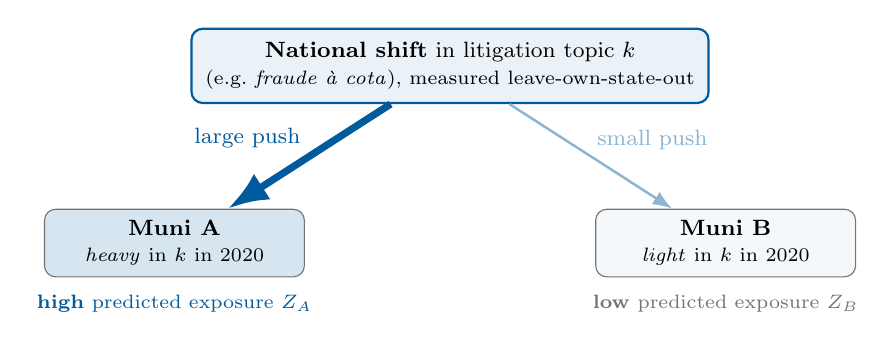
\begin{tikzpicture}[
  font=\footnotesize,
  wave/.style={draw=myblue, thick, rounded corners, fill=myblue!8, align=center, inner sep=5pt},
  muni/.style={draw=black!55, rounded corners, align=center, inner sep=4pt, minimum width=3.3cm},
  hi/.style={-{Latex}, myblue, line width=2.6pt},
  lo/.style={-{Latex}, myblue!45, line width=0.9pt},
]
  \node[wave] (nat) at (0,2.25) {\textbf{National shift} in litigation topic $k$\\ \scriptsize (e.g.\ \emph{fraude \`a cota}), measured leave-own-state-out};
  \node[muni, fill=myblue!16] (a) at (-3.5,0) {\textbf{Muni A}\\ \scriptsize \emph{heavy} in $k$ in 2020};
  \node[muni, fill=myblue!4]  (b) at (3.5,0)  {\textbf{Muni B}\\ \scriptsize \emph{light} in $k$ in 2020};
  \draw[hi] (nat) -- (a) node[midway,above left=-2pt]{large push};
  \draw[lo] (nat) -- (b) node[midway,above right=-2pt]{small push};
  \node[below=3pt of a, myblue]   {\scriptsize \textbf{high} predicted exposure $Z_A$};
  \node[below=3pt of b, black!55] {\scriptsize \textbf{low} predicted exposure $Z_B$};
\end{tikzpicture}
\end{center}
\vspace{2pt}
\centerline{\footnotesize The comparison is between municipalities pushed harder by \emph{identical} national trends.}
\smallskip
\footnotesize Two ingredients construct it: each municipality's 2020 caseload mix across litigation subjects, and the national shift in each subject measured leave-own-state-out. Both rest on a prior decision about which filings count as adversarial.
\end{frame}



\begin{frame}{The Adversarial Filter: What Counts as Treatment}
\hypertarget{src:adversarialfilter}{}
\footnotesize
Most electoral filings are mandatory paperwork: one candidacy registration (RRC/DRAP) and one finance account (\emph{presta\c{c}\~ao de contas}) per candidate. These move one-for-one with the candidate pool and carry no adversarial signal. Treatment keeps only genuine contests between political actors.
\smallskip

\begin{center}
\renewcommand{\arraystretch}{1.15}
\resizebox{0.94\linewidth}{!}{%
\begin{tabular}{L{6.0cm}L{6.0cm}}
  \toprule
  \cellcolor{bandvot}\textbf{Kept: adversarial contests} & \cellcolor{bandlaw}\textbf{Dropped: administrative / procedural} \\
  \midrule
  Propaganda, disinformation, right of reply & Candidacy registration (RRC / DRAP) \\
  Abuse of economic / political power (AIJE, AIME) & Campaign-finance accounts (\emph{presta\c{c}\~ao de contas}) \\
  Campaign-finance \& poll-conduct disputes & Vote tallying \& poll-worker admin \\
  Registration \& eligibility \emph{challenges} (\emph{impugna\c{c}\~ao}, inelegibilidade) & Procedural acts \& enforcement (citation, \emph{cumprimento}) \\
  Originating electoral crimes (vote-buying, \emph{a\c{c}\~ao penal}) & Voter-roll, party-internal, fiscal tail \\
  \bottomrule
\end{tabular}}
\end{center}
\smallskip

\begin{itemize}\itemsep3pt
  \item A filing is routed by subject and gated by class: it is kept on what it is \emph{about}, while its criminal status follows the procedural vehicle. A registration \emph{challenge} therefore survives even inside the mandatory registration class.
  \item What remains is \KeptAdversarialLawsuits{} adversarial filings, \KeptAdversarialPct\% of the \TotalAllLawsuits{} million total. Treatment is $\Delta\log(1+\ell_m)$, the 2020$\to$2024 change in this count per municipality.
\end{itemize}
\end{frame}



% ---------------------------------------------------------------------------
% A3 -- backs the "stays roughly flat and recomposes" claim (src:motivation)
% with the coverage-robust composition data. Count LEVELS are contaminated by
% the 2024 SIG coverage artifact, so nothing here is a volume trend: the LHS
% is a within-cycle SHAPE (each year normalized to its own total) and the RHS
% is all shares/ratios. Numbers come from litigation_composition.tex, generated
% by 01_descriptives.py -- nothing hard-coded.
% ---------------------------------------------------------------------------
\begin{frame}{Recomposition Without Aggregate Growth}
\hypertarget{app:recomp}{}
\footnotesize
The adversarial arena rearranges rather than expands. Filings run later in the cycle, leaving a fatter post-election tail; they escalate further, with more appeals and higher per-candidate intensity; and they tilt toward gender-quota fraud, while the broad topic mix barely moves.
\smallskip
\begin{columns}[T]
\begin{column}{0.50\linewidth}
\centering
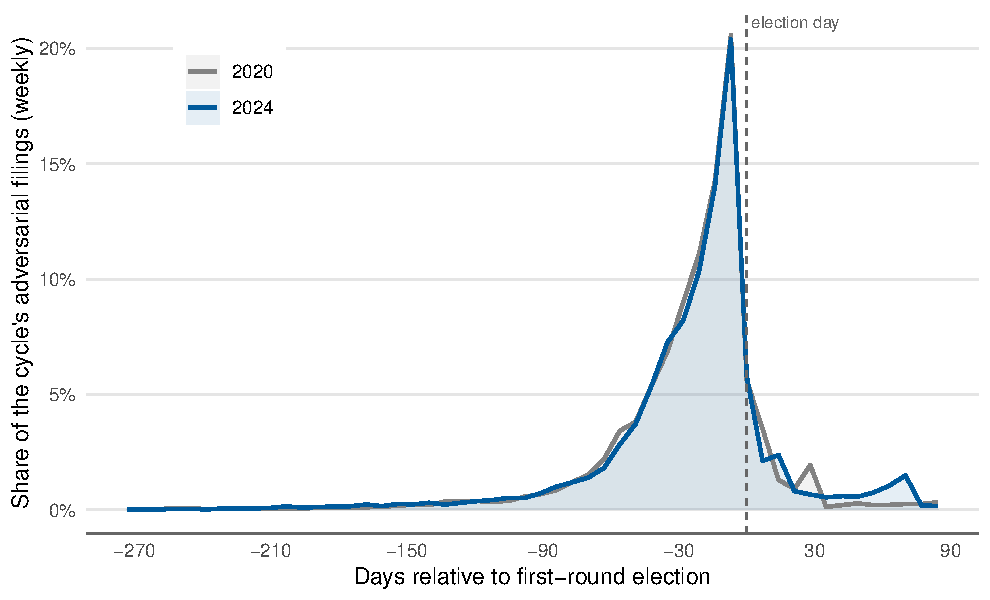
\includegraphics[width=\linewidth,height=0.44\textheight,keepaspectratio]{../figures/litigation_timing_shape.pdf}\\[4pt]
{\scriptsize\ns{Filings by week relative to the vote, each cycle normalized to its own total. Both peak in the final fortnight; 2024 (blue) carries the fatter post-vote tail.}}
\end{column}
\begin{column}{0.48\linewidth}
\centering
\resizebox{\linewidth}{!}{% Auto-generated by code/04_analysis/01_descriptives.py
% Do not edit manually -- rerun the generating script to update

\begin{tabular}{lcc}
\toprule\toprule
 & \textbf{2020} & \textbf{2024} \\
\midrule
\multicolumn{3}{l}{\textit{Within-adversarial composition (share of filings)}} \\
Campaign conduct & 0.520 & 0.516 \\
Information environment & 0.402 & 0.387 \\
Abuse / misuse of office & 0.060 & 0.074 \\
Eligibility \& ballot access & 0.018 & 0.022 \\
\midrule
\multicolumn{3}{l}{\textit{Character of the arena}} \\
Post-election filing share & 0.268 & 0.297 \\
Appeal escalation rate & 0.046 & 0.052 \\
Adversarial appeals per 1{,}000 candidates & 31.5 & 46.9 \\
\bottomrule\bottomrule
\end{tabular}
}\\[4pt]
{\scriptsize\ns{Topic shares (top) barely move, while the character rows (bottom) do: filings run later, appeal more, and per-candidate escalation rises by half.}}
\end{column}
\end{columns}
\smallskip
{\centering\scriptsize This matters for identification because the recomposition is national, and it reaches each municipality through that municipality's own 2020 topic mix. The same shift produces unequal local exposure, which is the variation the instrument uses.\par}
\smallskip
\end{frame}


\begin{frame}{Outcomes: Three Layers of the Contest}
\hypertarget{src:outcomes}{}
\small
The unit of analysis is the local election. We estimate whether adversarial litigation intensity changes the contest itself; who wins a given seat is not the object. Outcomes fall into three layers, each measured as a 2020--2024 change. Leveling and Barrier predict opposite signs in the first two layers, and the same sign in the third.
\vspace{10pt}
\begin{center}
\renewcommand{\arraystretch}{1.7}
\resizebox{\linewidth}{!}{%
\begin{tabular}{@{}l l c c@{}}
\toprule
 & Outcomes & \textcolor{mygreen}{Leveling predicts} & \textcolor{myred}{Barrier predicts} \\
\midrule
1\ \ Candidate supply & Entrants, women and non-white candidates, party count, field size & broader pool & fewer, safer names \\
2\ \ Voter response & Turnout, blank and null votes & engagement sustained & withdrawal \\
3\ \ Contest outcome & Top-two margin, effective number of candidates, incumbency advantage & ambiguous & consolidation \\
\bottomrule
\end{tabular}}
\end{center}
\vspace{10pt}
{\centering\footnotesize Only layer 2 discriminates. A narrower contest is consistent with either face, so the face is assigned on the ballot.\par}
\end{frame}


% ----------------------------------------------------------
\section{Empirical Strategy}


\begin{frame}{Specification: 2SLS on a 2016 Baseline}
\hypertarget{src:spec}{}
\small
First stage (OLS), instrumenting the change in litigation intensity:
\[
\underbrace{\Delta\log(1+\ell_{m})}_{\text{endogenous}} \;=\; \alpha + \beta\, \bZ + \mathbf{X}_m'\boldsymbol{\gamma} + \delta_{\text{UF}(m)} + \varepsilon_m
\]
Second stage (2SLS), ANCOVA on the 2016 pre-window baseline:
\[
Y_{m,2024} \;=\; \alpha + \tau\, \widehat{\Delta\log(1+\ell_{m})} + \lambda\, Y_{m,2016} + \mathbf{X}_m'\boldsymbol{\gamma} + \delta_{\text{UF}(m)} + u_m
\]
\begin{itemize}\itemsep1pt
  \item $\ell_m$ = adversarial lawsuits (originating filings in the cycle) resolved to the municipality of origin; $\Delta$ = first difference 2024$-$2020.
  \item The outcome enters in levels on a clean 2016 baseline. $Y_{m,2016}$ predates the 2020 exposure shares, so it is a true pre-treatment lag; $\lambda$ is freely estimated and $\tau$ reads the 2024 level holding 2016 fixed.
  \item \hypertarget{src:fd}{}ANCOVA is preferred to first differences because municipal outcomes barely persist. First differences pin $\lambda=1$, over-differencing and attenuating the estimate, so FD serves as an appendix check . Outcomes with no clean 2016 analog remain in FD.
  \item $\mathbf{X}_m$ = 6 pre-determined controls (log population, urbanization, log income p.c., 2010 higher-education share, 2020 valid-vote volume, 2016 top-two margin); $\delta_{\text{UF}(m)}$ = state FE (\NClusters{} of 27 UFs). SE clustered by state.
\end{itemize}
\end{frame}


\begin{frame}{Constructing the Instrument: Shares $\times$ Shifts}
\hypertarget{src:instrument}{}
\footnotesize
The instrument combines a pre-determined 2020 exposure share with a leave-own-state-out national shift, at the subject level (\NSubjectsKept{} kept TSE subjects; no family aggregation is imposed on $\bZ$).
\smallskip

\textbf{Shares:} each municipality's 2020 adversarial-subject mix, fixed two cycles before 2024 outcomes.
\[
s_{m,k,2020} \;=\; \frac{\text{adversarial lawsuits of subject } k \text{ in } m,\ 2020}{\text{all adversarial lawsuits in } m,\ 2020},
\qquad \sum_k s_{m,k,2020}=1.
\]
\textbf{Shifts:} each subject's log caseload growth, summed over all other states.
\[
g_{\text{UF}(m),\,k} \;=\; \log\!\bigl(1 + L_{-\text{UF},\,k,\,2024}\bigr) - \log\!\bigl(1 + L_{-\text{UF},\,k,\,2020}\bigr),
\qquad L_{-\text{UF},\,k,\,t} = L^{\text{nat}}_{k,t} - L^{\text{own-UF}}_{k,t}.
\]
\textbf{Instrument:} the portfolio-weighted predicted exposure, one number per municipality.
\[
\bZ \;=\; \sum_{k} \; \underbrace{s_{m,k,2020}}_{\text{share (pre-determined)}} \;\cdot\; \underbrace{g_{\text{UF}(m),\,k}}_{\text{shift (other states)}}
\]
\smallskip
\begin{itemize}\itemsep2pt
  \item Leaving out the own state removes local litigation shocks from the shift. A municipality's shift excludes its whole state, so every municipality in a state shares the same per-subject shift and state fixed effects absorb it. Identification therefore comes from within-state variation in the 2020 shares, and the adjudication locus (the zone) sits inside the state.
  \item The variation is off subjects that diffuse across states, such as jurisprudence, MPE priorities and party legal strategy, rather than off local politics. The same $\bZ$ is carried into the executive and legislative designs.
\end{itemize}
\end{frame}

\input{frames/src_identbrief_talk.tex}

% ----------------------------------------------------------
\section{Results}
\input{frames/src_firststage_talk.tex}

\begin{frame}{Candidates, Voters, and What the Contest Produces}
\hypertarget{src:story}{}
\small
An election is produced by two behaviors: candidates decide whether to run and how to campaign, and voters decide whether to turn out and how to mark the ballot. We isolate the contest's judicial dimension and ask how each side responds and what the two jointly produce.
\vspace{-4pt}
\begin{center}
\scalebox{0.94}{
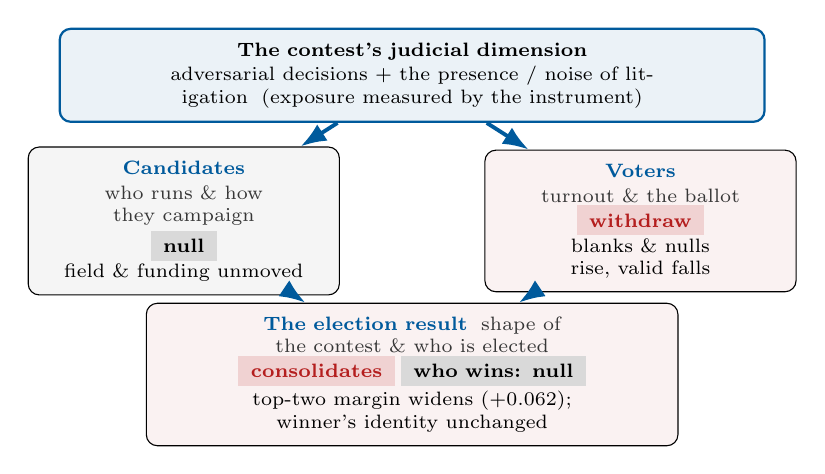
\begin{tikzpicture}[
  font=\scriptsize,
  exp/.style={draw=myblue, thick, rounded corners, fill=myblue!8, align=center, inner sep=5pt, text width=8.6cm},
  eng/.style={draw, rounded corners, align=center, inner sep=5pt, minimum height=1.75cm, text width=3.6cm},
  res/.style={draw, rounded corners, align=center, inner sep=5pt, minimum height=1.4cm, text width=6.4cm},
  flow/.style={-{Latex}, myblue, line width=1.4pt},
]
  \node[exp] (exp) at (0,2.25)
    {\textbf{The contest's judicial dimension}\\[1pt]adversarial decisions $+$ the presence / noise of litigation \;(exposure measured by the instrument)};
  \node[eng, fill=mygray!8] (cand) at (-2.9,0.4)
    {\textcolor{myblue}{\textbf{Candidates}}\\[1pt]\ns{who runs \& how they campaign}\\[1pt]
     \colorbox{mygray!30}{\textbf{\,null\,}}\\[1pt]
     {field \& funding unmoved}};
  \node[eng, fill=myred!6] (vot) at (2.9,0.4)
    {\textcolor{myblue}{\textbf{Voters}}\\[1pt]\ns{turnout \& the ballot}\\[1pt]
     \colorbox{myred!20}{\textcolor{myred}{\textbf{\,withdraw\,}}}\\[1pt]
     {blanks \& nulls rise, valid falls}};
  \node[res, fill=myred!6] (res) at (0,-1.55)
    {\textcolor{myblue}{\textbf{The election result}} \;\ns{shape of the contest \& who is elected}\\[1pt]
     \colorbox{myred!20}{\textcolor{myred}{\textbf{\,consolidates\,}}}\;\colorbox{mygray!30}{\textbf{\,who wins: null\,}}\\[1pt]
     {top-two margin widens ($\MarginCoef$); winner's identity unchanged}};
  \draw[flow] (exp) -- (cand);
  \draw[flow] (exp) -- (vot);
  \draw[flow] (cand) -- (res);
  \draw[flow] (vot) -- (res);
\end{tikzpicture}
}
\end{center}
\vspace{-4pt}
\footnotesize The candidate side is quiet while voters withdraw where an incumbent is defended. The consolidation is general across seat types and comes from the electorate re-allocating toward the leader rather than from candidates being removed. A narrower contest does not by itself name a face, so the barrier reading rests on the ballot, and the council race is null throughout.
\end{frame}

\input{frames/src_spine1_talk.tex}


\begin{frame}{The Consolidation Favors the Incumbent}
\hypertarget{src:favored}{}
\small
Consolidation reinforces whoever is already ahead, and the 2024 mayoral field identifies who that is descriptively, before any regression. Profiling candidates by within-race vote rank shows that the winner and the runner-up part on political standing rather than demographics. The front-runner is a sitting incumbent roughly five times as often; on gender, race, education and age the top two are near-twins.
\smallskip
\begin{center}
\scriptsize
\resizebox{!}{0.23\textheight}{% Auto-generated by code/04_analysis/10_candidate_rank_profile.py (2024 mayoral)
% Do not edit manually -- rerun the generating script to update

\begin{tabular}{lccc}
\toprule\toprule
 & \textbf{Winner} & \textbf{Runner-up} & \textbf{Rest of} \\
 & \scriptsize{(1st)} & \scriptsize{(2nd)} & \scriptsize{field} \\
\midrule
\multicolumn{4}{l}{\textit{Political standing}} \\
\rowcolor{mylight}
\quad Incumbent (won this seat last cycle) & 42.2 & 7.7 & 1.1 \\
\quad Prior election winner & 65.1 & 48.9 & 28.5 \\
\quad First-time candidate & 25.0 & 32.7 & 42.6 \\
\midrule
\multicolumn{4}{l}{\textit{Demographics}} \\
\quad Female & 13.2 & 17.1 & 16.4 \\
\quad Non-white & 33.9 & 35.7 & 39.0 \\
\quad Higher education & 64.2 & 62.6 & 65.7 \\
\quad Age (years) & 50.0 & 51.0 & 51.5 \\
\midrule
$N$ candidates & 5,560 & 5,331 & 4,141 \\
\bottomrule\bottomrule
\end{tabular}
}
\end{center}
\smallskip
\takeaway{Because the top two are demographically interchangeable, widening the margin between them entrenches incumbency, which is a politically rather than demographically defined trait. This is mechanically why the vote-weighted gender and race composition of winners cannot move: what the consolidation protects is incumbency. \ns{Descriptive shares by vote rank; no causal content.}}
\end{frame}

\input{frames/src_representation_talk.tex}
\input{frames/src_gender_talk.tex}
\input{frames/src_candidates_talk.tex}
\input{frames/src_voterballot_talk.tex}
\input{frames/src_seathet_talk.tex}

% ----------------------------------------------------------
\section{Robustness}
% ============================================================

\begin{frame}{Robustness: Four Threats and Their Verdicts}
\hypertarget{src:robustness}{}
\footnotesize
The design rests on a few concentrated shocks and an extensive-margin first stage, so credibility comes from a battery of targeted checks rather than from averaging many independent shifters.
\smallskip
\renewcommand{\arraystretch}{1.05}
\begin{center}
\scriptsize
\begin{tabular}{@{}p{2.7cm} p{5.9cm} c @{\hskip 5pt}p{2.1cm}@{}}
\toprule\toprule
\textbf{Threat} & \textbf{Check} & \textbf{Verdict} & \textbf{Appendix} \\
\midrule
The identifying variation is not what we claim &
Reduced form survives dropping every zero-litigation municipality and a presence dummy; count-native Poisson and NegBin confirm the weak intensive margin is a real null. &
\tick &
\,  \\
\midrule
The treatment definition drives the result &
Invariant across log1p, IHS, level, rate and binary definitions. Only weak-first-stage transforms lose significance, which is a weak-IV symptom rather than counter-evidence. &
\tick &
 \\
\midrule
The inference overstates precision &
Consolidation clears the weak-IV-robust AR bootstrap and the BHJ/AKM exposure-robust SE, whose CI still excludes zero at the outer bound. First differences provide a conservative bracket. &
\tick &
\,  \\
\midrule
The result is multiple testing &
Clears Holm and Benjamini--Hochberg at 5\% (Romano--Wolf at 10\%: $p=.059$) and loads onto a combined consolidation index, with no favorable family cut. Pre-trend placebos are clean throughout. &
\tick &
\,  \\
\bottomrule\bottomrule
\end{tabular}
\end{center}
\footnotesize The consolidation clears every threat; the withdrawal result remains tentative, clearing the exposure-robust SE but not the AR bootstrap. The nulls remain null under each check.
\end{frame}

\input{frames/src_pretrend_talk.tex}

% ----------------------------------------------------------
\section{Conclusion}
% ============================================================

\begin{frame}{Findings by Confidence Tier}
\hypertarget{src:findings}{}
\footnotesize
On the clean 2016 baseline the evidence sorts into four tiers of confidence:
\medskip
\begin{itemize}\itemsep1pt
  \item[\textcolor{myred}{\rule{1.2ex}{1.2ex}}] \textbf{Robust.} The mayoral race consolidates: the top-two margin widens ($\MarginCoef$, $p=\MarginP$), the winner's share rises ($\WinShareCoef$) and the runner-up's falls ($\RunnerUpCoef$). It clears the weak-IV-robust AR wild-cluster bootstrap (margin $p=\ARMarginP$, runner-up $p=\ARRunnerUpP$), the BHJ/AKM exposure-robust SE (CI $\ERMarginCI$ excludes zero), and multiplicity correction at 5\% by Holm and Benjamini--Hochberg, with Romano--Wolf, the most conservative of the three, clearing at 10\% ($p=.059$).
  \item[\textcolor{myred!55}{\rule{1.2ex}{1.2ex}}] \textbf{Tentative.} Voters disengage on the same ballot: mayoral blank ($\BlankCoef$) and null ($\NullCoef$) votes rise and valid votes fall, concentrated in contested seats, while compulsory turnout stays pinned. Significant under conventional and exposure-robust inference (exposure-robust $p=\ERBlankPbhj$) but not the AR bootstrap ($p=\ARBlankP$).
  \item[\textcolor{mygray}{\rule{1.2ex}{1.2ex}}] \textbf{Precise nulls.} Descriptive representation and renewal, the entrant typology, elastic and education-stratified turnout, campaign finance, and the entire legislative side are all tightly bounded around zero. The consolidation's cost belongs here as well: the runner-up's loss splits evenly by gender ($\RUGapCoef$, $p=\RUGapP$).
  \item[\textcolor{mygray!55}{\rule{1.2ex}{1.2ex}}] \textbf{Exploratory.} The winner's gain lands on male front-runners ($\MaleWinSharePerSDSigned$~pp, $p=\MaleWinShareP$) with the female winner's share flat, but the differential test does not clear ($p=\WinGapP$) and these outcomes sit outside the declared family. The data suggest the direction without establishing it.
\end{itemize}
\medskip
\footnotesize The candidate side is quiet while some voters withdraw, so the consolidation is the electorate re-allocating votes toward the leader rather than candidates being removed. The two halves of the claim carry different weight: the consolidation is robust, while the barrier reading sits one tier down because it rests on the ballot.
\end{frame}


\begin{frame}{Limitations}
\hypertarget{src:limitations}{}
\small
Four considerations bound the reach of the claim.
\medskip
\begin{enumerate}\itemsep4pt
  \item \textbf{Few effective shocks.} Identification rests on $K_{\text{eff}}=\KeffRotemberg$ effective shocks, with \RotPropagandaPct\% of the weight on propaganda subjects, and on \NClusters{} clusters. A many-shock law of large numbers \ns{\citep{borusyak2022}} does not apply, so the design is defended on the exogeneity of the 2020 shares rather than on shock count. That exogeneity is only partly supported: on unclustered tests, \GpsCovFail{} of \GpsNTopics{} tested topic shares correlate with the baseline controls, and \GpsMarginPtFail{} predict the 2016$\to$2020 margin change.
  \item \textbf{Extensive-margin identification.} The first stage moves the treatment on the extensive margin, so the per-unit-of-volume magnitude is not well identified even though the existence and sign of the effect are. The estimate is a local effect for onset compliers.
  \item \textbf{The face assignment is tentative.} The consolidation is robust, but which face produced it is assigned by the open-versus-contested split, and that split turns on ballot movement in contested seats that clears conventional and exposure-robust inference without clearing the AR bootstrap. If that ballot movement failed to replicate, the consolidation would survive and the barrier reading would not.
  \item \textbf{Aggregate, not case-level.} The treatment is municipal-level litigation intensity, not any single suit, so the design speaks to the aggregate climate of judicialization a race faces rather than to the outcome of a specific case.
\end{enumerate}
\end{frame}


% ----------------------------------------------------------
\section{References}
\begin{frame}[allowframebreaks]{References}
\hypertarget{src:references}{}
\footnotesize
\bibliographystyle{plainnat}
\bibliography{biblio}
\end{frame}


\end{document}
